 %------------------------------------------------------------------------------
% Template file for the submission of papers to IUCr journals in LaTeX2e
% using the iucr document class
% Copyright 1999-2013 International Union of Crystallography
% Version 1.6 (28 March 2013)
%------------------------------------------------------------------------------

\documentclass[preprint]{iucr}              % DO NOT DELETE %\documentclass{iucr}              % DO NOT DELETE THIS LINE
\usepackage{bm}
% \usepackage{graphicx}
% \usepackage{tabularx}
% \usepackage{subfigure}
% \usepackage{afterpage}
% \usepackage{sansmath}
\usepackage{mathtools}
% \usepackage{parskip}
% \usepackage{tikz}
% \usepackage{tikzorbital}
% \usepackage{setspace}
% \usepackage{xcolor}
% \usepackage{amssymb}
% \usepackage{bm}
\usepackage{amsmath}
% \usepackage{fancyhdr}
% \usepackage{rotating}
% \usepackage{siunitx}
\usepackage[hyphens,spaces,obeyspaces]{url}
\usepackage{color}

\newcommand{\todo}[1]{{\color{red}[TODO: "#1'']}}
\newcommand{\manuel}[1]{{\color{red}[Manuel: #1]}}
\newcommand{\inblue}[1]{{\color{blue}#1}}
\newcommand{\inred}[1]{{\color{red}#1}}
\newcommand{\ingreen}[1]{{\color{green}#1}}



     %-------------------------------------------------------------------------
     % Infobrmation about journal to which submitted
     %-------------------------------------------------------------------------
     \journalcode{S}              % Indicate the journal to which submitted
                                  %   A - Acta Crystallographica Section A
                                  %   B - Acta Crystallographica Section B
                                  %   C - Acta Crystallographica Section C
                                  %   D - Acta Crystallographica Section D
                                  %   E - Acta Crystallographica Section E
                                  %   F - Acta Crystallographica Section F
                                  %   J - Journal of Applied Crystallography
                                  %   M - IUCrJ
                                  %   S - Journal of Synchrotron Radiation

\begin{document} % DO NOT DELETE THIS LINE

     %-------------------------------------------------------------------------
     % The introductory (header) part of the paper
     %-------------------------------------------------------------------------

     % The title of the paper. Use \shorttitle to indicate an abbreviated title
     % for use in running heads (you will need to uncomment it).


\title{
Simulating applications with Diaboloid mirrors}

\cauthor[a]{Manuel}{Sanchez del Rio}{srio@esrf.eu}{address if different from \aff}
\author[b]{Valeriy V.}{Yashchuk}
\author[b]{Ian}{Lacey}
\author[b]{Kenneth A.}{Goldberg}
\author[b]{Howard A.}{Padmore}

\aff[a]{European Synchrotron Radiation Facility, 71 Avenue des Martyrs F-38000 Grenoble \country{France}}
\aff[b]{Advanced Light Source, LBNL, Berkeley CA, USA}


\begin{synopsis}
xxxxx
\end{synopsis}

\begin{abstract}
The Diaboloid is a reflecting surface that convert a spherical wave to a cylindrical wave. This complex surface may find application in new ALS-U bending magnet beamlines or in other  beamlines that now exploit todoidal optics for astigmatic focusing. We describe here the implementation of the Diaboloid mirrors in the Oasys environment with some results of  simulations. 
\end{abstract}

\section{Motivation}

%Hi Manolo,  here is a quick set of notes related to motivation for the work and the background............why we went with a 2:1 partially aberration corrected system, why this was OK in 2000, why it started not to be OK in 2013 when the horizontal source size was reduced by 3 (we take a factor of 2 reduction in brightness), and why we need to do something very different........the Diaboloid...........when we reduce the horizontal source size by a factor of 6 with ALSU.  I also tried to answer the question why does anyone care about bending magnet sources..........ie. why do we care about a diaboloid as a new type of optical element.  I also put in a few words about the daunting task of making such an optical element, but there are methods on the horizon.  One is to use computer generated hologram interferometry.  I believe there are several other possibilities as well.  I'm happy to write a summary as well.  Perhaps its also worth expanding a bit on the importance of the conical approximation as it possibly is easier to make.  I also think that in 1 case, showing the deviation of the surface from the toroid makes sense..............in the paper with Wayne which I sent, I was surprised by how small a difference it was.   Cheers, Howard

In the development of synchrotron radiation sources, brightness has always been a key metric, and as such the emphasis has always been on undulators.  A secondary consideration has been the development of the bending magnets. These white light sources hold key advantages for a range of x-ray experiments, such as Laue diffraction, dispersive EXAFS and other experiments which take advantage of a wide bandwidth.  In other areas, the agility in photon energy offered by a monochromatized bending magnet radiation is a key advantage.  Now with the advent of 4th generation MBA synchrotron sources, bending magnet sources are becoming even more attractive for a segment of synchrotron experiments.  However a key technical challenge is how to maintain the brightness of these sources while imaging a significant horizontal aperture.  In undulator sources we have the luxury of using only tangentially curved optics for focusing in both horizontal and vertical planes.  For bending magnet sources, to collect a reasonable horizontal aperture, we have to use sagittaly curved optics.  This could be as in a crystal monochromator with a sagittally curved 2nd crystal, or with a sagitally focusing cylindrical or toroidal mirror.  At ALS we decided to adopt toroidal mirrors for our protein crystallography beamlines, due to the robustness of the system.  In order to preserve the brightness, it was found that if we had a system with a tangentially collimating pre-mirror and a toroid mirror downstream of the crystal monochromator, if we focused from infinity in the vertical direction and from the real source in the horizontal direction with 2:1 demagnification,  astigmatic coma aberrations vanished \cite{MacDowell2004}. At the time, the rms horizontal source size was 100 $\mu$m and the residual aberrations were far less.  Following an upgrade of the ALS in 2013, the horizontal beam size was reduced to 40 $\mu$m  rms \cite{Steier_2014}. The residual aberrations were still tolerable, but cause around a factor of 2 decrease in brightness.  With the current ALS-U project, the new lattice will produce a horizontal beam size of 7 $\mu$m rms.  At this value the residual aberrations of our 2:1 aberration correcting toroidal mirror solution are now longer adequate.

This has led us to consider new types of optics which will preserve the brightness of bending magnets sources, with particular importance for MBA-style 4th generation sources.   
For many applications we need good monochromatization and good tunability.  This is provided by the classical collimated double crystal monochromator.  The task therefore is to design an optical element which can accept light from infinity in the vertical direction and from the real source in the horizontal direction and focus it to a point.  The parabolic mirror produces a beam that is parallel in the vertical direction, so that each infinitesimal segment of the beam will land on a unique part of the mirror.  It is evident therefore that along the tangential direction the mirror should be parabolic, but for rays away from the axis, the limiting shape will be elliptical. The purpose of this paper is to describe this new surface type, and to demonstrate how this system focuses for real applications. We have named this surface the Diaboloid, to indicate the complexity of the surface.   Although the idea is to replace the toroids in our protein crystallography superbend beamlines with this new type of mirror, the application goes further than this, as now we can demagnify much more strongly than in the previous 2:1 aberration corrected toroid case.  One such example is in a high pressure beamline where currently we focus the beam using the normal 2:1 demagnification system and then demagnify to a few micron focus using a K-B mirror pair.  In an updated system using the Diaboloid, the K-B mirror will be redundant, and we will be able to directly focus to around a 3 $\mu$m spot size, increasing flux, increasing image quality and decreasing complexity.

It is important to note that fabrication of such complex surfaces has been impossible, at the slope error level that we require.  For a typical application at ALS, the mirror to source distance is 20 m, and so with a 10 $\mu$m vertical source size, including angle doubling on reflection, an angular error budget of half of the angular size of the source, the tangential slope error tolerance is 0.13 $\mu$rads.  The sagittal slope error tolerance is 18 $\mu$rads.  The tangential tolerance is extremely challenging, but mainly limited by metrology.  Local area correction, and stitching interferometer-based metrology have led to 1D curved optics with significantly smaller slope errors \cite{Yamauchi2002}.  The problem is that current high accuracy metrology techniques cannot work with steeply curved optics.  One possible solution is to use metrology based on computer generated hologram (CGH) reference beams, as now widely used in free form optics fabrication. In addition, we have investigated an approximation to the diaboloid which should be much easier to manufacture and test, but which gives similarly high performance. 

%TODO: from Howard email May 21st 2020:
% Actually I think there is a sentence of 2 missing from the intro. 
%
% As it says there is history to recount............2:1 toroid was OK for als1..........when it was upgraded we lose a factor of 2 in brightness (now)............when we have alsu we would use a lot more.   ALS upgrade happened over several years and came into action in 2013.....but in 2009, due to the fact that we knew we were going to lose brightness. we started looking at alternatives to the toroid (Mckinney reference).  The gain from the Diaboloid at that time was too small for the increase in cost / complexity, but with ALSU the loss in brightness would be too high and we really need to find an alternative................hence due to need, and due to the fact that we think that these surfaces can now be made. we have revisited the diaboloid

% old intro (removed)
%Most optical surfaces used in optical systems used as reflectors can be classified in one large family (conic) plus toroidal surfaces. Conic surfaces are quadratic surfaces. Some familiar conic mirrors are: ellipsoidal mirrors (perfect point-to-point focusing), or paraboloids (perfect point-to-point focusing with one focus in the infinity). Hyperboloids may be used when one point (source or image) is virtual. In some cases these 2D focusing surfaces are approximated by surfaces of circular section, that are simpler to produce. Toroidal mirrors can approximate ellipsoidal and paraboloidal mirrors for 1D focusing. The toroid is a quartic (fourth order) surface. Toroids present spherical and coma aberrations. The toroids can be use in astigmatic focusing, with different focal points in the meridional and sagittal plane. An useful case is when the meridional focus is at infinity: a point source is converted into a collimated beam in one direction (tangential) and focused beam in the other (sagittal). This finds important applications in beamline optics when the beam is collimated in one direction for matching better the monochromator aperture, and then has to be refocused to the sample. When the beam is represented by a wavefront, a cylindrical wave coming from the monochromator has to be converted Numerical implementation of the propagation of a wavefront in vacuum is fundamental for many synchrotron radiation applications related to modeling beamline optics and data analysis. Here the most commonly used methods and implementations are described. into a spherical wave collapsing to the focal point. When using a toroid, this conversion is not perfect as it has aberrations. The Diaboloid is the surface that makes this conversion exactly. 

%Many aspects of the Diaboloid mirrors including the pioneering ideas, different mathematical descriptions, and suggested applications are related to work performed at the LBNL. A short history is in Ref.~\cite{Goldberg2020}.

We created a tool in the Oasys environment \cite{codeOASYS} that implements numerically the Diaboloid surfaces (Section~\ref{sec:DiaboloidEqs}) and its approximations (Section~\ref{sec:approximations}): the toroid and the parabolic-cone. A new widget is created in Oasys (Section~\ref{sec:oasys}) that can be plugged into the ray-tracing code SHADOW \cite{codeSHADOW}. 
In the stand-alone tool in Oasys we adopted a solution of the Diaboloid that include an approximation (we call it "basal-plane approximation"). In addition, the exact solution can be computed externally and loaded in Oasys. We analyzed the validity of this approximation (Section~\ref{sec:testing}).
We used this application to make simulations of the ALS beamline 12.2.2 (Section~\ref{sec:beamline}) where the Diaboloid is compared to other surface approximations for ALS and ALS-U. We also treated in Section~\ref{sec:scan} a possible upgrade of this beamline using high demagnification and analyze the feasibility of using the simpler parabolic-cone to replace diaboloids. Final remarks are given in Section~\ref{sec:summary}.

\section{Equation of the Diaboloid surface}
\label{sec:DiaboloidEqs}

For practical purposes want to define the Diaboloid surface as a function of the focal distances $p,q$ ($p$ is the source-mirror distance, $q$ is the mirror-image distance) and the grazing incidence angle $\theta$. The Diaboloid can be placed in two configurations: i) to convert a spherical wave into a cylindrical wave (we also refer that to point-to-segment focusing or Diaboloid Type I) and ii) to convert a cylindrical wave into a spherical one (or segment-to-point focusing or Type II). We will need to obtain the numerical mesh as a function of a "mirror-related coordinate system" ($X,Y,Z$), with origin in the center of the mirror, one axis ($Y$) tangent to the Diaboloid surface origin in the direction of the beam propagation, another axis ($X$) tangent to the Diaboloid surface origin in the direction perpendicular of the beam propagation, and the third axis ($Z$) is outward pointing perpendicular to $X$ and $Y$. Therefore the surface in its explicit form needed for being evaluated numerically is $Z(X,Y)$ with $X \in [-W/2, W/2]$ and $Y \in [-L/2, L/2]$ with $L$ the mirror length and $W$ the mirror width. The mirror length is sampled in $N_Y$ points and the mirror width in $N_X$ points, therefore the height or elevation of a point is $Z_{i,j}=Z(X_i,Y_j)$.

The exact expression of the Diaboloid in the "mirror-related coordinate system" is possible (see  Refs.~\cite{Valeriy2020a}, \cite{Valeriy2020b}) but is extremely long. It has been implemented in a Mathematica code \cite{lacey} to produce the numeric mesh. The Diaboloid surface equation takes a simple form \cite{Valeriy2020a} when expressed in a coordinate system ($x,y,z$) that we call "canonical-mirror system". This system has the same origin as ($X,Y,Z$) (the mirror center), the $x$ axis is parallel to $X$, but $y$ is parallel to the direction of the beam after reflection (therefore forming an angle $\theta$ with $Y$), and $z$ is perpendicular to $x$ and $y$ thus also forming an angle $\theta$ with $Z$ (see Fig.~\ref{fig:frame}).

\begin{figure}[h]
\centering
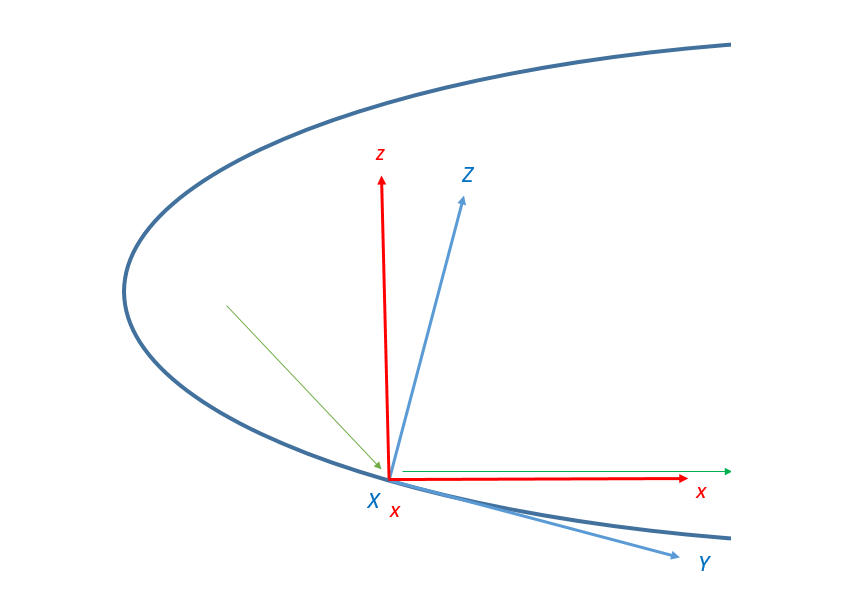
\includegraphics[width=0.5\textwidth]{figures/diaboloid_frame.png}
\caption{\label{fig:frame}Schematic of the reference frames in use: "mirror-related coordinate system" $(X,Y,Z)$ and "mirror-canonical system" $(x,y,z)$}
\end{figure}

The equation of the Diaboloid (point-to-segment focusing or Type I) in the canonical-mirror system is first deduced in Ref.~\cite{Valeriy2020a} and takes the form (Eq.(12) in Ref.~\cite{Valeriy2020b}):

\begin{equation}
\label{eqn:diaboloidV}
z(x,y) = p \sin2\theta- \sqrt{ 4 p^2 \sin^4\theta - 2 (p \cos2\theta+q) (y + p  \cos2\theta) + 2 (p+q) (p \cos2\theta + q - \sqrt{x^2 + (q-y)^2}) }.
\end{equation}


It is also deduced in Ref.~\cite{Goldberg2020} in this form:
\begin{equation}
\label{eqn:diaboloidK}
z(x,y) = p \sin2\theta - \sqrt{(c^2 + q^2 - s^2) - 2 (s  + q) y - 2 c \sqrt{x^2 + (q-y)^2}},
\end{equation}
with $c=p+q$ and $s=p\sin\theta$. It is easy to demonstrate that these two equations are equivalent.

Once we have the equation of the Diaboloid in the canonical-mirror reference system, one has to rotate it an angle $\theta$ around the $x$ axis to retrieve the equation in the mirror-related coordinate system. The expresion obtained is extremely long (see Appendix in Ref.~\cite{Valeriy2020b}). It can be defined in Mathematica as an analytical function, ready for numerical calculations of the desired Diaboloid surface profiles.

In most practical case the grazing incidence $\theta$ is small, therefore we can pass from the canonical-mirror system to the mirror-related coordinates by substraction of the basal plane that is tangent to the Diaboloid surface at the origin. This can be done numerically after evaluating the surface in the canonical-mirror system using Eqs.~\ref{eqn:diaboloidV} or \ref{eqn:diaboloidK}. Calling $Z'(X',Y')$ the result after removing numerically the basal plane, we suppose (to be justified in Section~\ref{sec:testing}) it is a good approximation to the exact solution $Z(X,Y$) because $X'=X, Y'\approx Y, Z'=z - \theta Y' \approx Z$. 

It can be shown that the meridional section of the Diaboloid is a parabola, and the sagittal section is an ellipse (Refs.~\cite{Goldberg2020},\cite{Valeriy2020a}).

\section{Surfaces that approximate the diaboloid}
\label{sec:approximations}

\subsection{Toroid}
The simplest approximaton of the Diaboloid is the toroid, with optical radii $R_m$ and $R_s$ (in the meridional and sagittal directions, respectively) given by the focusing conditions (Coddington equations): 

\begin{equation}
\label{eqn:radii}
\frac{1}{p} = \frac{2 }{\sin\theta R_r};~~~~~~
\frac{1}{p} + \frac{1}{q} = \frac{2\sin\theta}{ R_s}.
\end{equation}

The tangential circle (at $X=0$), ans sagittal circle ($Y=0$) will be

\begin{equation}
\label{eqn:toroidTS}
Z(0,Y) = R_t - \sqrt{R_t^2 - Y^2};~~~~~~~~
Z(X,0) = R_s - \sqrt{R_s^2 - X^2},
\end{equation}
and the toroidal surface is the addition of both profiles: 
\begin{equation}
\label{eqn:toroid}
Z(X,Y) = Z(X,0) + Z(0,Y) = 
R_t + R_s - \sqrt{R_s^2 - X^2}
- \sqrt{R_t^2 - Y^2}.
\end{equation}

\subsection{Parabolic-cone}
An approximation to the Diaboloid better than the toroid consist in taking a parabola in the meridinal direction and then adding a circle in the sagittal direction. However, the sagittal circle must have different radius for the different $Y$ coordinates. This surface that will be called "parabolic-cone" has been proposed and deduced in Ref.~\cite{Valeriy2020c}. It can be expressed as (Eq.~(17) in \cite{Valeriy2020c}):
\begin{equation}
\label{eqn:parabolicCone}
Z(X,Y) = Y \tan\theta - 2 \sec\theta \tan\theta
\sqrt{Y p \cos\theta + p^2} + 2 p \sec\theta \tan\theta +
k_1 + k_2 Y - \sqrt{(k_1 + k_2 Y)^2 - X^2},
\end{equation}
where $k_1$ and $k_2$ are
\begin{equation}
k_1 = \frac{p q \cos\theta \sin2\theta}{p+q};~~~~~~
k_2 = \frac{\sin2\theta(q-2p\cos^2\theta)}{2(p+q)}.
\end{equation}

The variation of the sagittal radius versus $Y$  (Eq. (2)\ in \cite{Valeriy2020c})
\begin{equation}
\label{eq:sagRadius}
R_s(Y) = \frac{2  p \sin\theta}{p + q} (q - Y)   \sqrt{Y / p + \cos^2\theta}
\end{equation}
is not linear. The variation of the sagittal radius in a cone is linear, therefore, strictly speaking, our "parabolic-cone" is not a cone. 

\begin{figure}[h]
\centering
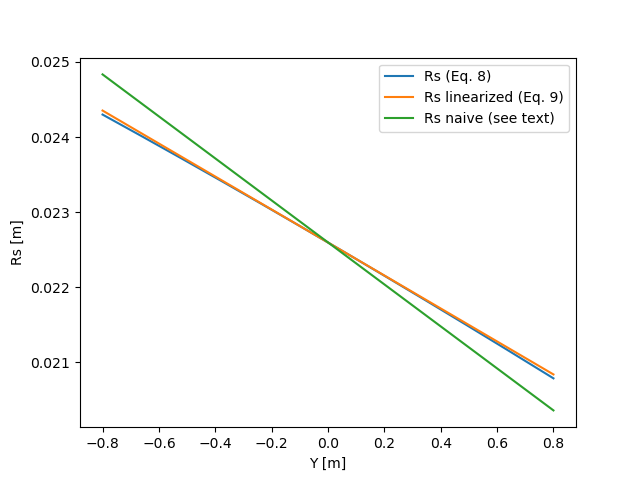
\includegraphics[width=0.65\textwidth]{figures/sagittalradius.png}
\caption{\label{fig:sagittalRadius}Radius in the sagittal direction as a function of the tangential coordinate $Y$ for the parabolic-cone (Eq.~\ref{eq:sagRadius}), its linearized value (Eq.~\ref{eq:sagittalRadiusLinearized}), and a naive estimation (see text), using $p$=18.8~m, $q$=8.075~m and $\theta$=2~mrad.
}
\end{figure}

In Fig.~\ref{fig:sagittalRadius} we have compared the variation of the radius as shown in Eq.~\ref{eq:sagRadius} with its linearization
% evaluate at x=0 this: https://www.wolframalpha.com/input/?i=%28derivative+%5B2+p+%28q+-+x%29+S+sqrt%28x+%2F+p+%2B+C%5E2%29+%2F+%28p%2Bq%29%2C+x%5D%29
\begin{equation}
\label{eq:sagittalRadiusLinearized}
R_s(Y) = \frac{p q \sin2\theta  }{p + q} + \frac{q \tan\theta - 2 p \sin\theta \cos\theta}{p + q} Y.
\end{equation}


A first comment is the central sagittal radius $R_s(Y=0)=p q \sin2\theta / (p+q)$ is very close, but not exact to the one given by the Coddington equation $R_s^c=2 p q \sin\theta / (p+q)$. The second comment is that the variation of the sagittal radius given by Eq.~\ref{eq:sagittalRadiusLinearized} is significantly different (see Fig.~\ref{fig:sagittalRadius}) to a "naive" variation generated the applying the Coddington equation at every point in $Y$ (that "sees" the source and image at distances $p'=\sqrt{(-p \cos\theta - Y)^2 + (p \sin\theta)^2}$ and $q'=\sqrt{(q \cos\theta - Y)^2 + (q \sin\theta)^2}$, respectively, and angle $\theta'=\arcsin(p \sin\theta / p')$).


\section{Implementation in Oasys of the Diaboloid and related surfaces}
\label{sec:oasys}

We have implemented a code to create a numerical mesh describing the different surfaces where the shown equations are used: Diaboloid (Eq.~\ref{eqn:diaboloidK} and Eq.~\ref{eqn:diaboloidV}), parabolic-cone (Eq.~\ref{eqn:parabolicCone}) and toroid (Eq.~\ref{eqn:toroid}). These surfaces correspond to the Type I (point-to-segment) focusing scheme. The Type II surfaces are calculated by exchanging the $p$ and $q$ values, and flipping the $Y$ array. In the case of Diaboloid surfaces, the passage to ($X,Y,Z$) is done by detrending a plane as discussed before. Two options are allowed, in the first the plane has an equation $Z=\theta Y$ and in the second one the plane is the result of the best fit of the Diaboloid to a plane. We recall that this is an approximation to the Diaboloid in the ($X,Y,Z$) frame, but as it will be discussed below, it is usually a good approximation but requires the use of grazing incidence. A system analyzed in Ref.~\cite{Yashchuk2019} shows a case where this approximation cannot be used.  

The different equations are codded in Python and interfaced in a Oasys Widget. This interface asks for the type of surface to calculate, with different geometries (Diaboloid, parabolic cone or toroid), focusing arrangement (point-to-segment or segment-to-point) and, in the case of Diaboloid, the Eq. used (we label "K" when they come from Ref.~\cite{Goldberg2020} and "V" from Ref.~\cite{Valeriy2020b}). Other controls permit to define the sampling of the $X$ and $Y$ axes and the detrending option. The interface also allows to remove the toroid from the calculated surface. This option may be useful compare the Diaboloid with the toroid. The surface is written in a {\tt hdf5} formatted file, as it is standard for Oasys surfaces. This format allows to input easily the numerical surface into several Oasys applications, like the ray-tracing tool ShadowOui \cite{codeSHADOWOUI}, and also wave optics codes (SRW, Wofry). Because of that, the "Diaboloid" widget is found in the "Syned" add-on. A view of the interface is in Fig.~\ref{fig:widget}.

\begin{figure}[h]
\centering
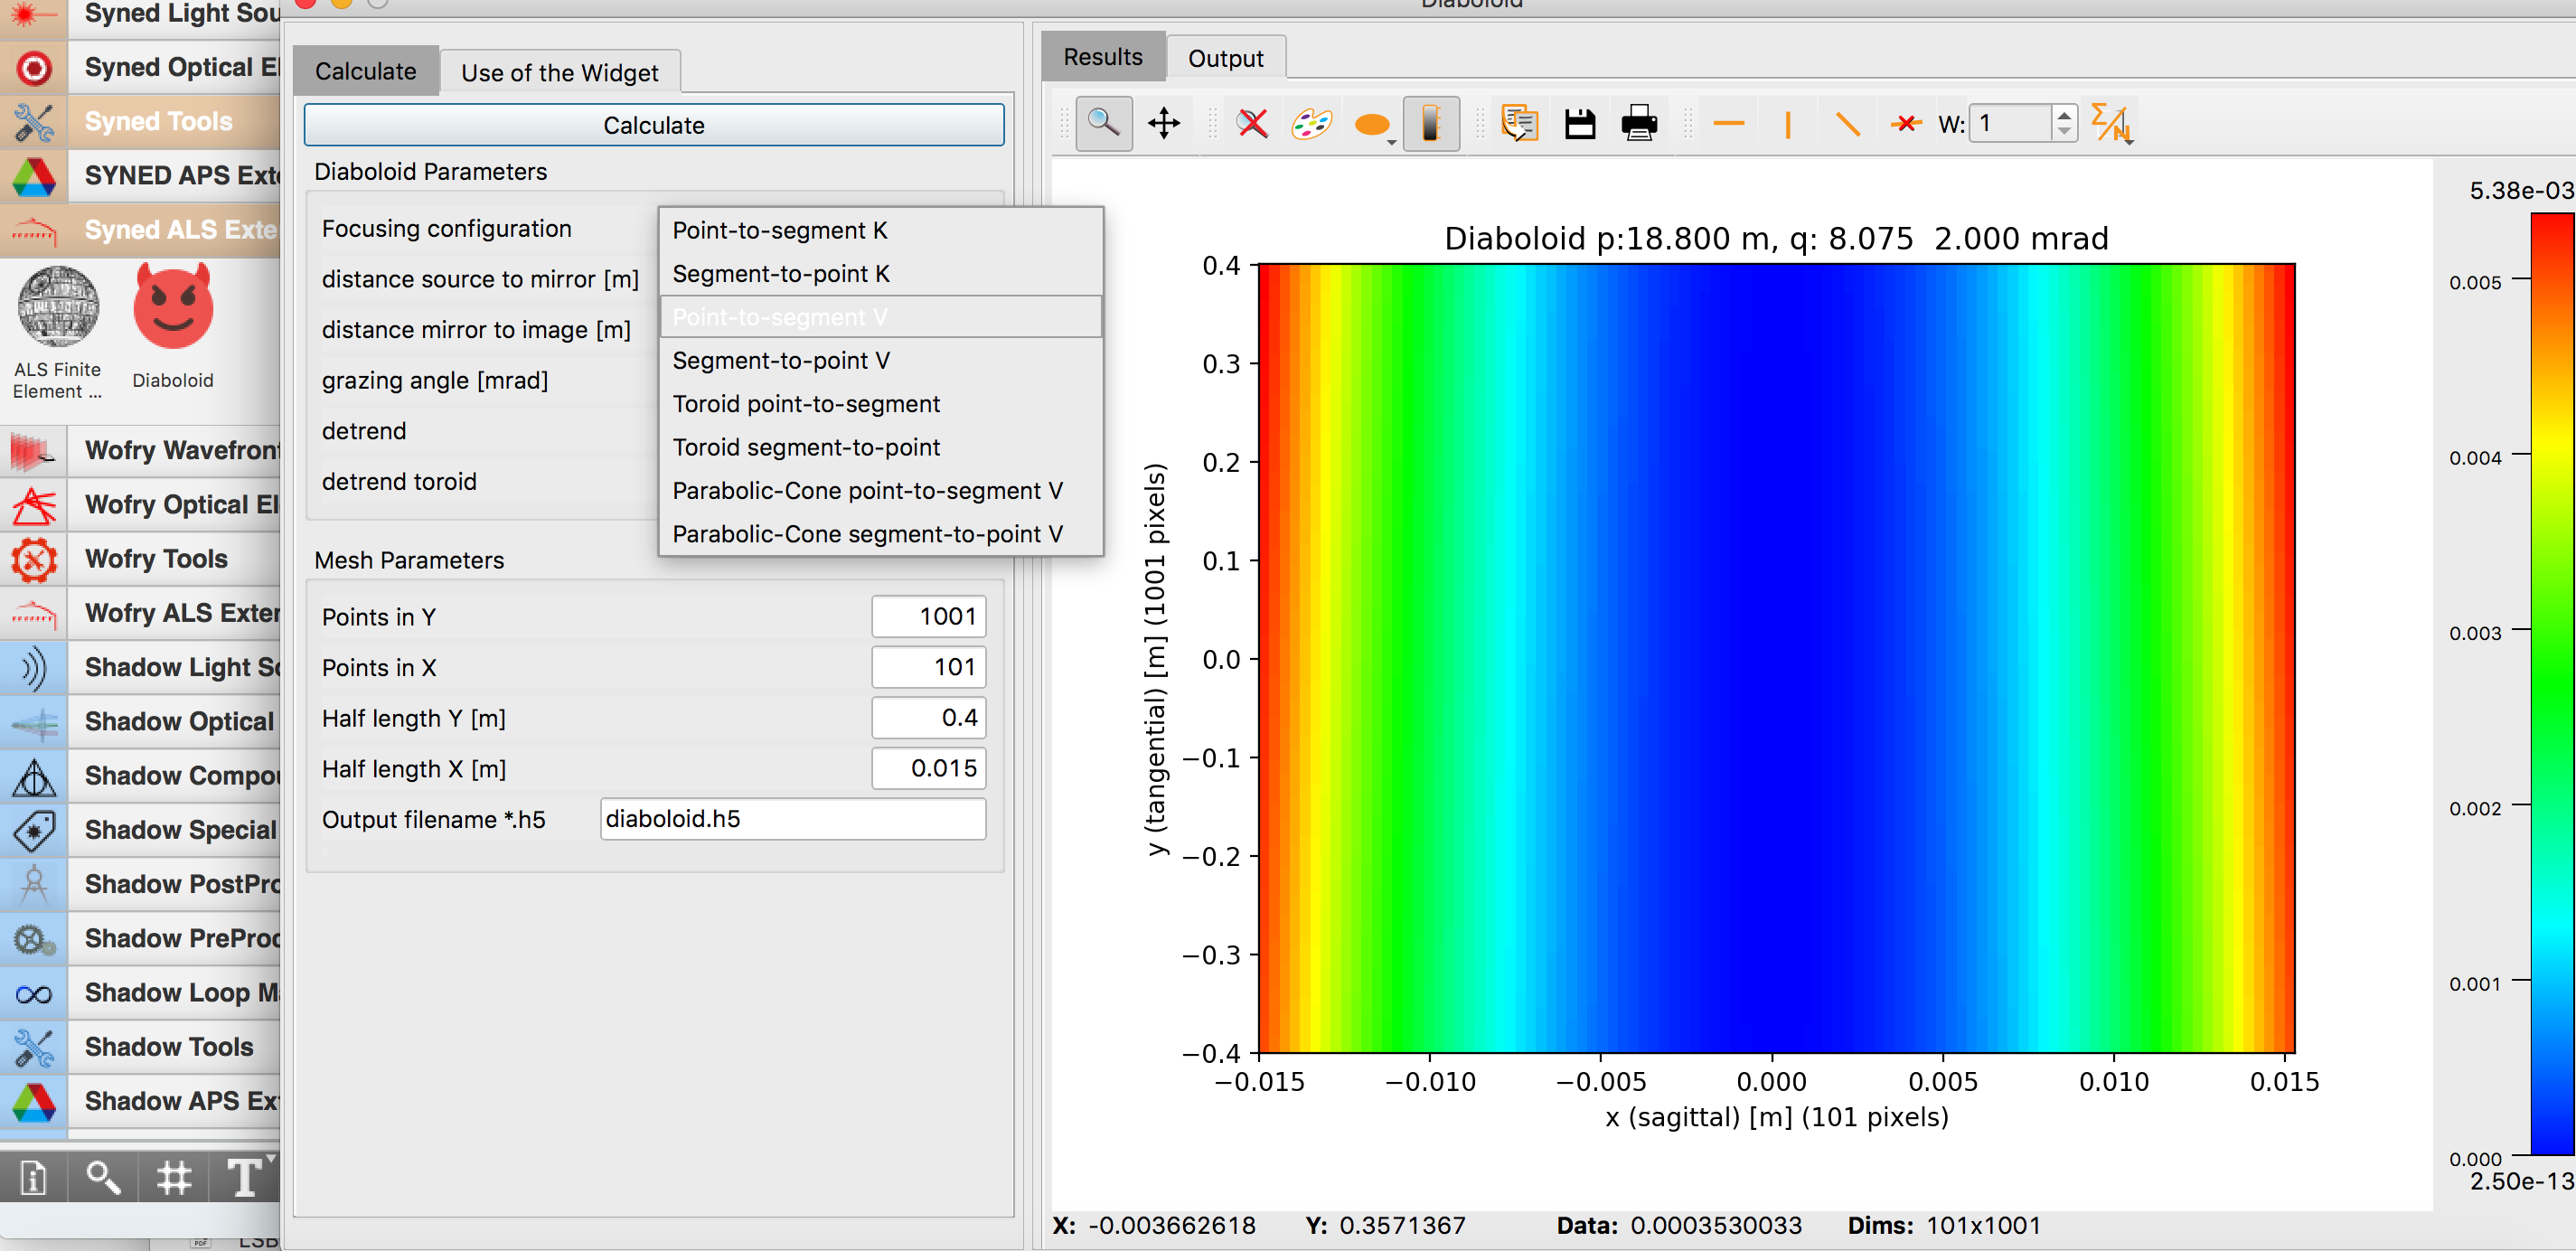
\includegraphics[width=0.7\textwidth]{figures/widget.png}
\caption{\label{fig:widget}View of the interface to create the numerical sampling of the Diaboloid and related surfaces ("Diaboloid" widget in Oasys/Syned) }
\end{figure}

To use the created surface with the ray-tracing tool, the Diaboloid widget has to be connected to a "Plane mirror" via the "Oasys Surface Data Converter" found in ShadowOui that will automatically convert the file in {\tt hdf5} format to SHADOW format. The reason of using a Plane mirror is because we add the numeric surface to an existing one. If we select the "Plane" the numeric mesh is added until a flat surface $Z(X,Y)$=0. Another possibility is to use the ShadowOui "Toroidal Mirror" and add the Diaboloid but created with the option "detrend Toroid" activated.  

\section{Testing the Diaboloid surfaces by ray-tracing}
\label{sec:testing}

In this section we perform ray tracing using a single Diaboloid with the purpose to test the accuracy of the calculations. The simpler case of point-to-segment (Type I) configuration is chosen, with $p$=29.3~m, $q$=19.53~m and $\theta$=4.5~mrad. A point source is created with divergence large enough to fully illuminate the mirror dimensions: 
length $L$=0.2~m, and width $W$=0.02~m.

\begin{figure}[h]
\flushleft
~~~~~~a)~~~~~~~~~~~~~~~~~~~~~~~~~~~~~~~b)~~~~~~~~~~~~~~~~~~~~~~~~~~~c)~~~~~~~~~~~~~~~~~~~~~~~~~~~~d)\\
\centering
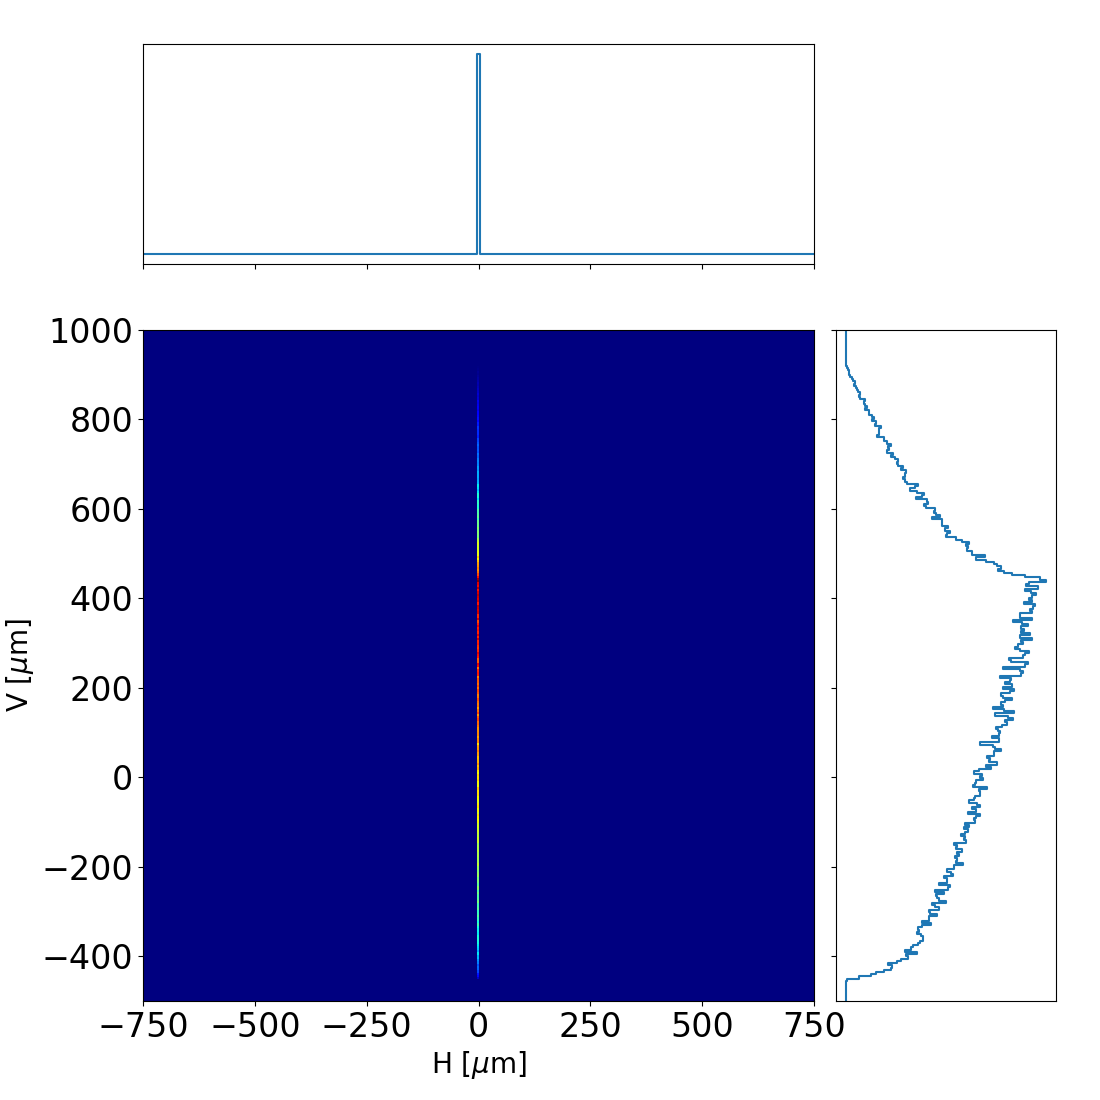
\includegraphics[width=0.22\textwidth]{figures/p2s_V.png}
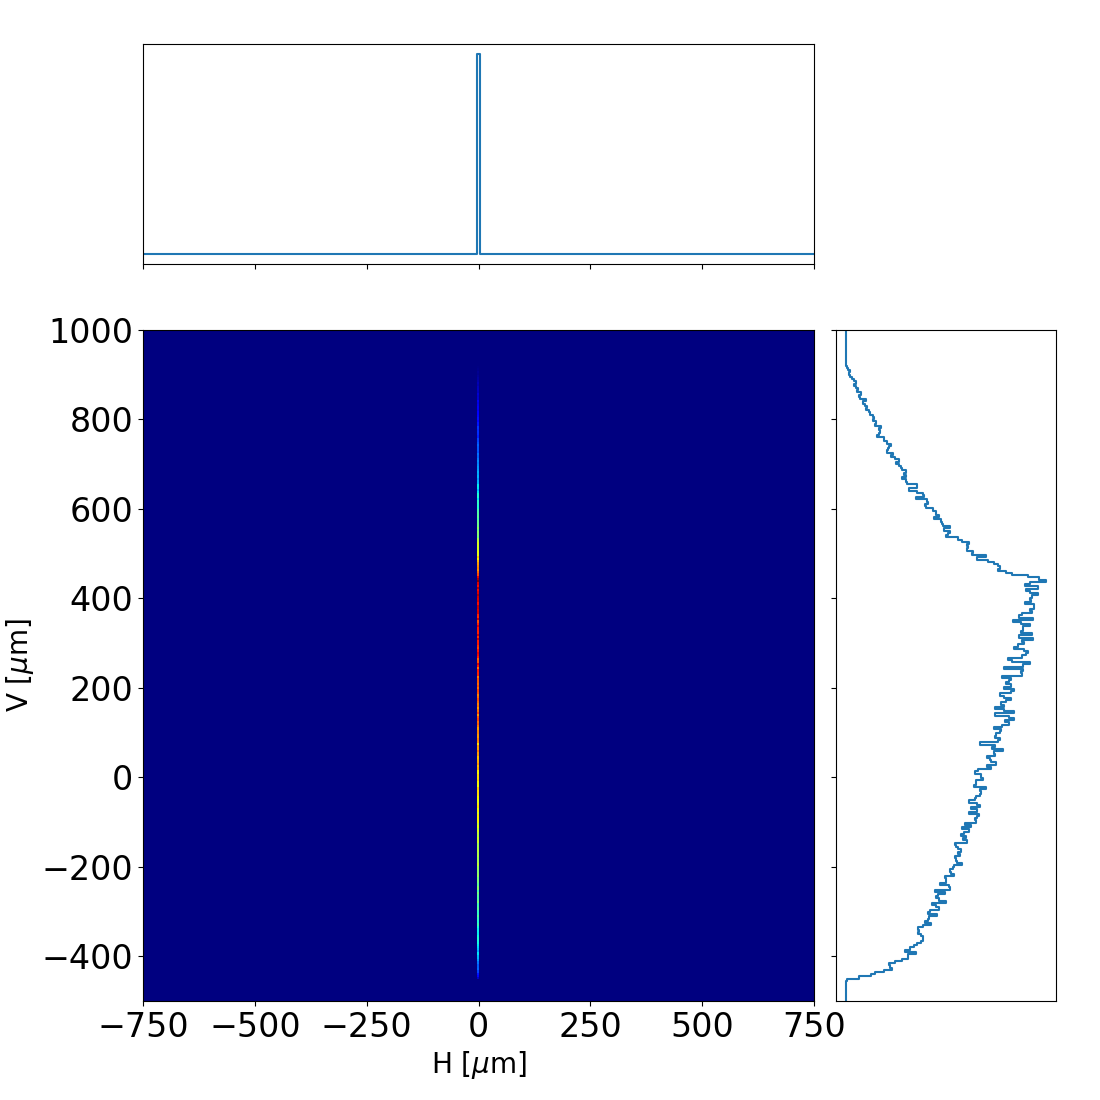
\includegraphics[width=0.22\textwidth]{figures/p2s_K.png}
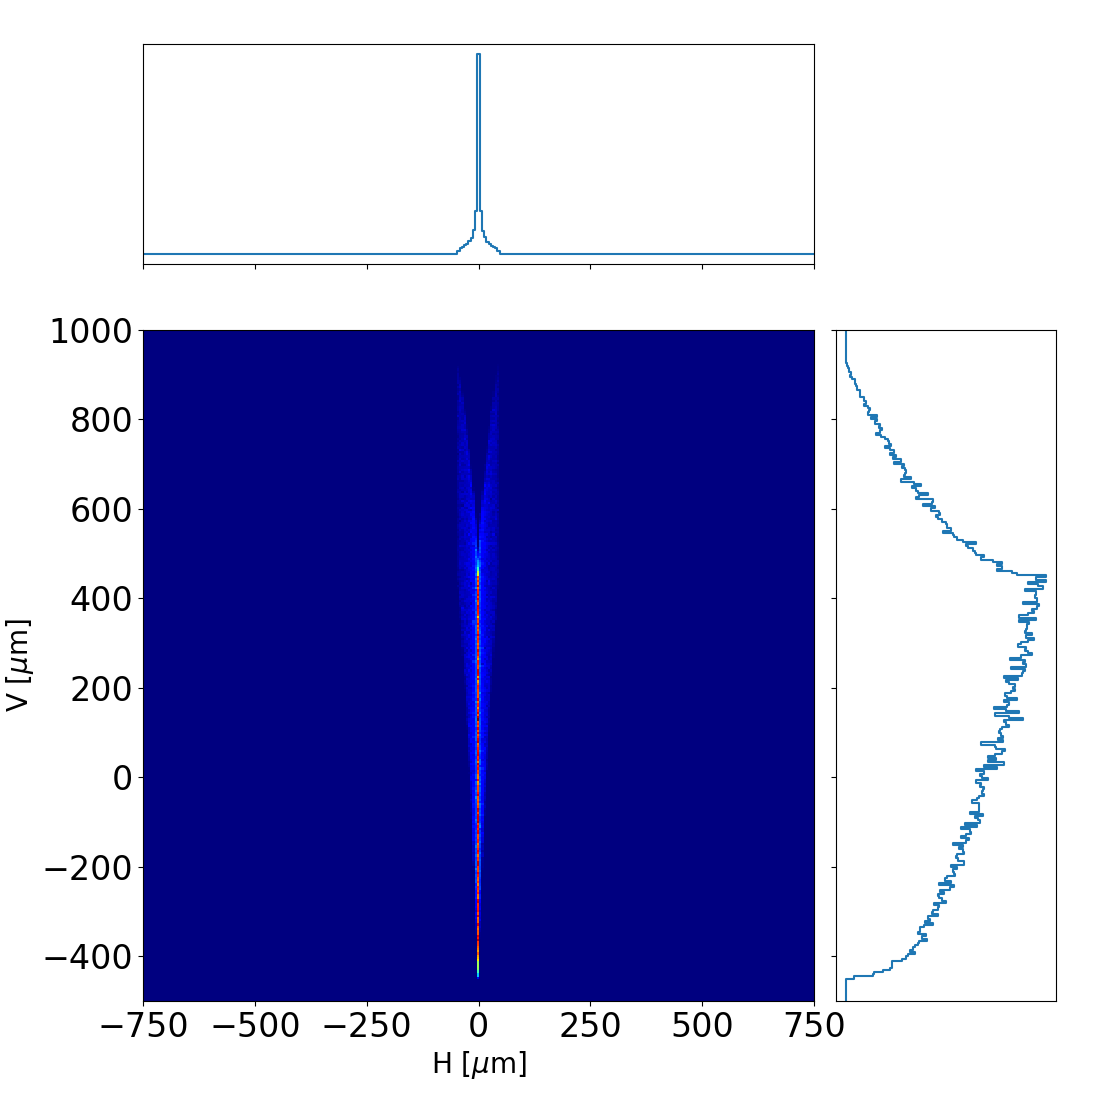
\includegraphics[width=0.22\textwidth]{figures/p2s_parabolic-cone.png}
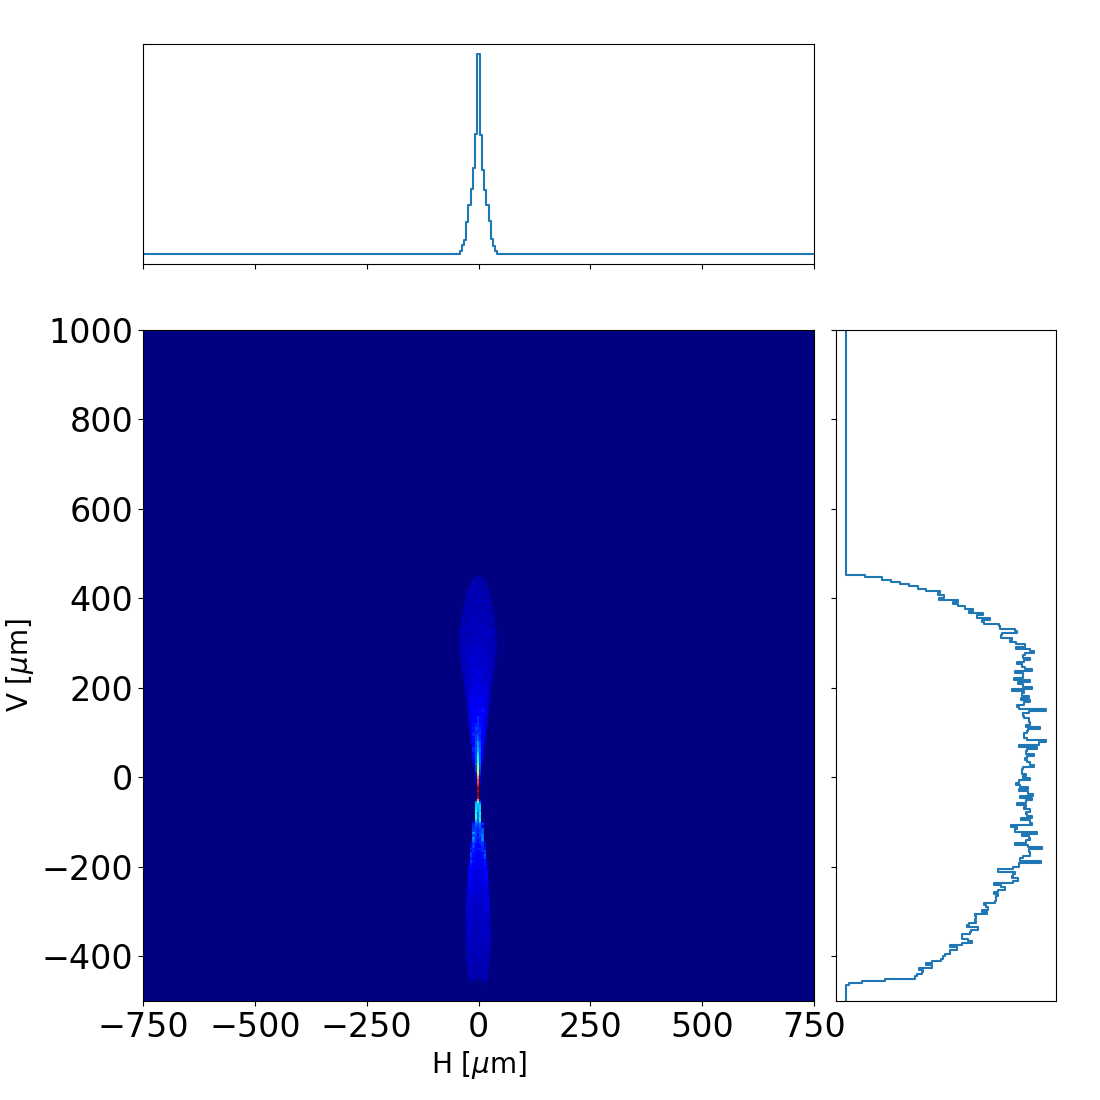
\includegraphics[width=0.22\textwidth]{figures/p2s_toroid.png}

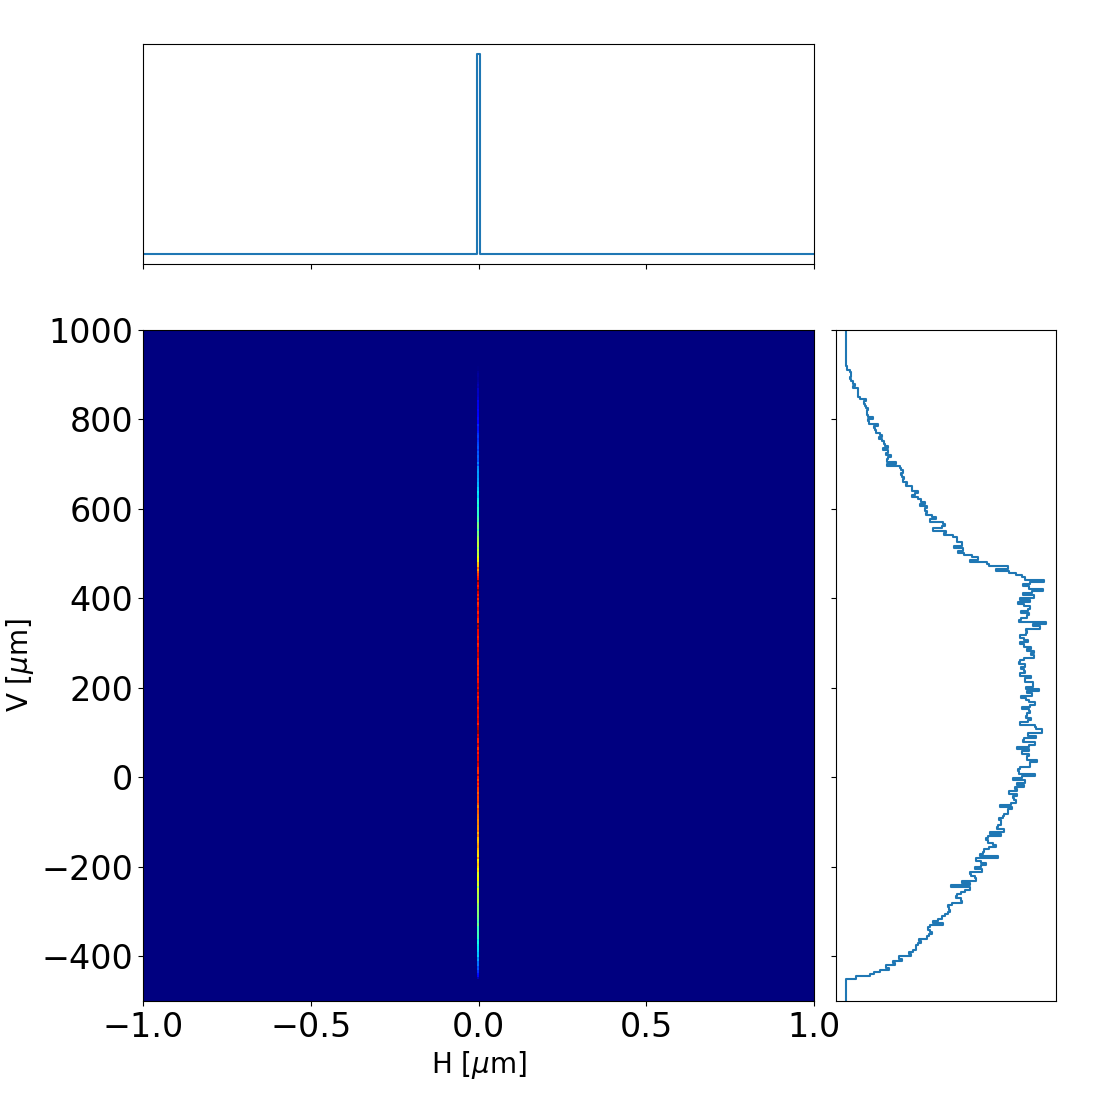
\includegraphics[width=0.22\textwidth]{figures/p2s_V_z.png}
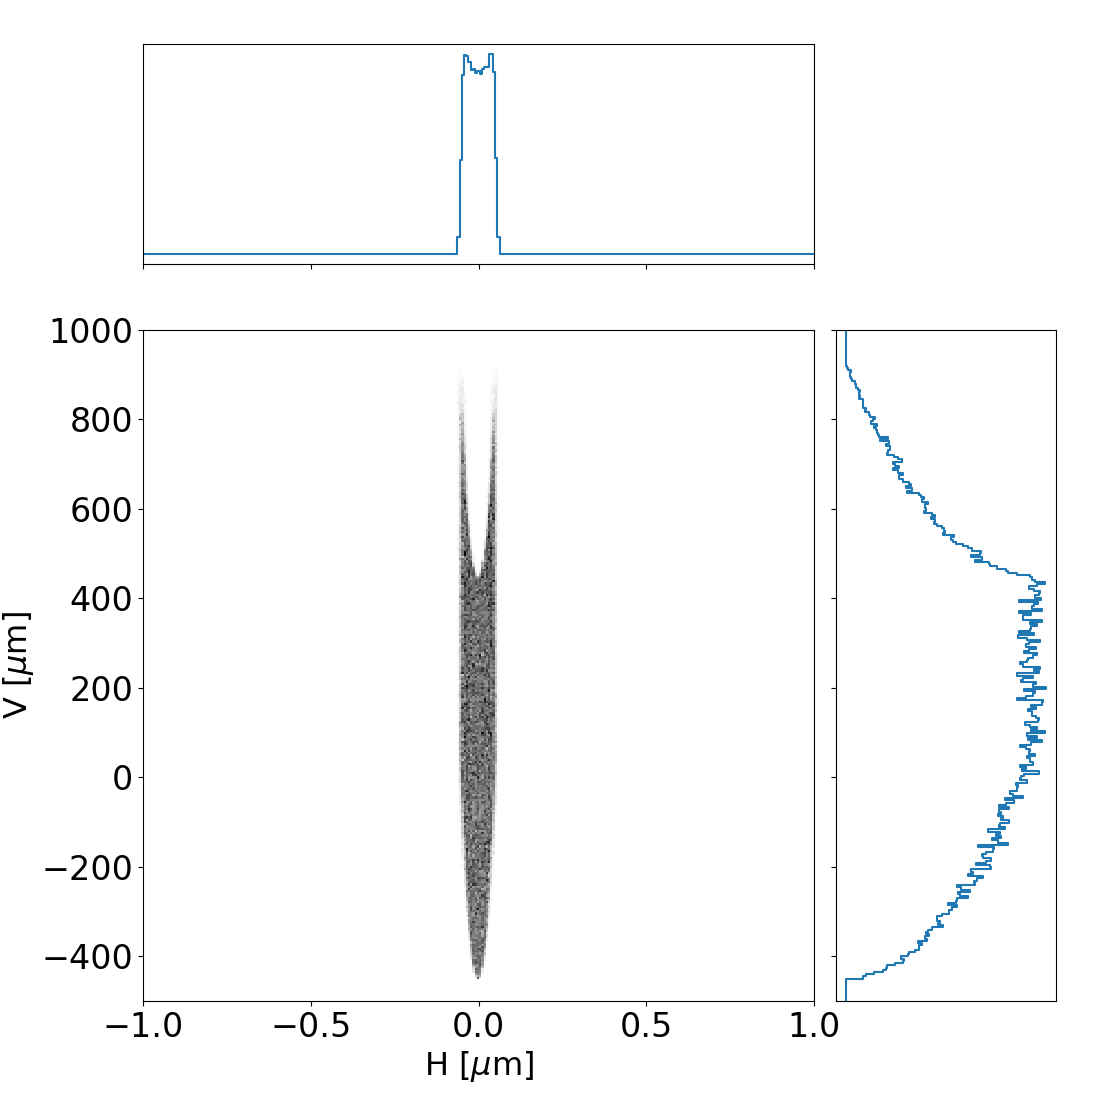
\includegraphics[width=0.22\textwidth]{figures/p2s_K_z.png}
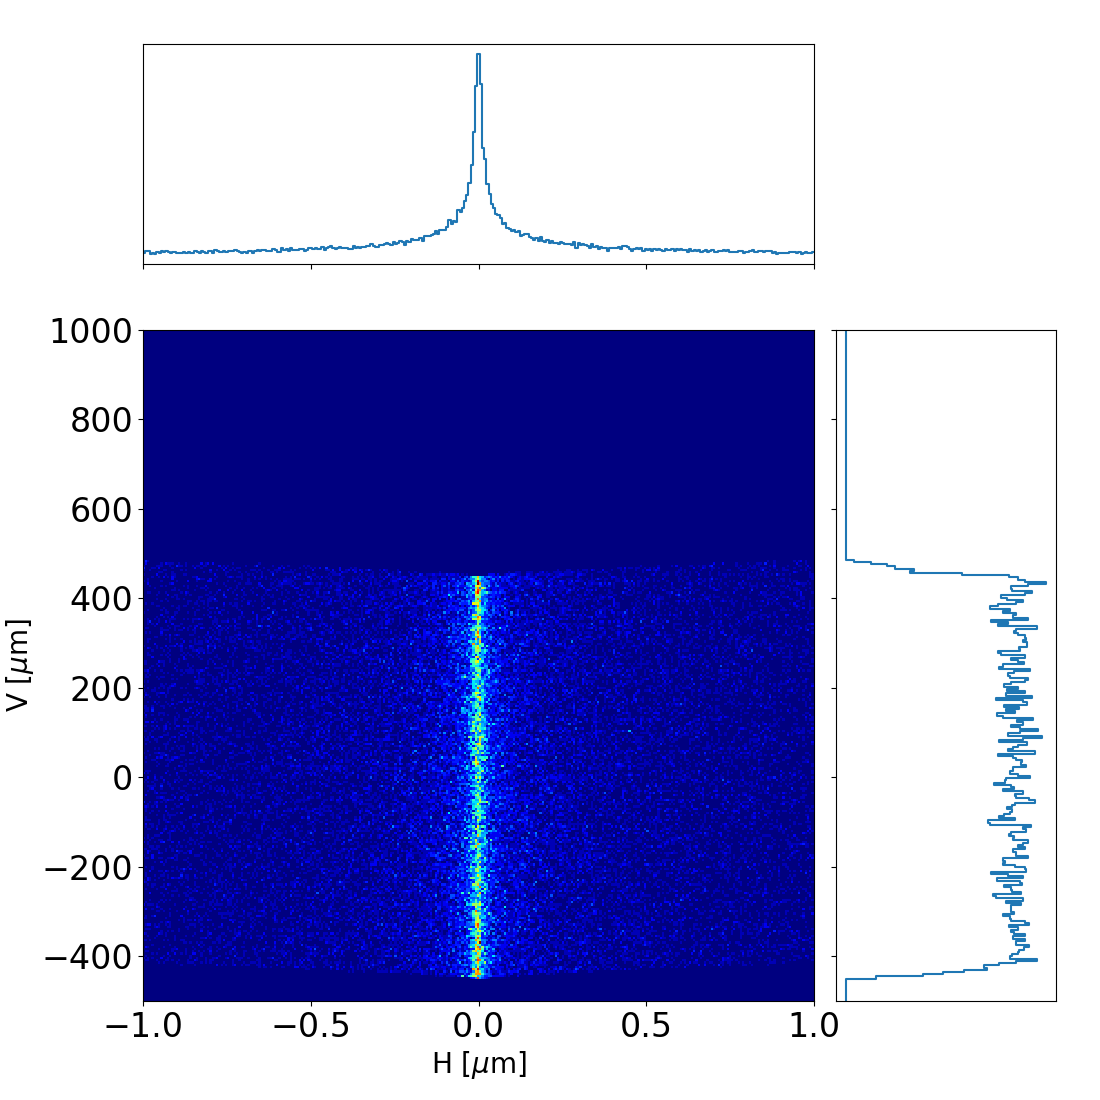
\includegraphics[width=0.22\textwidth]{figures/p2s_parabolic-cone_z.png}
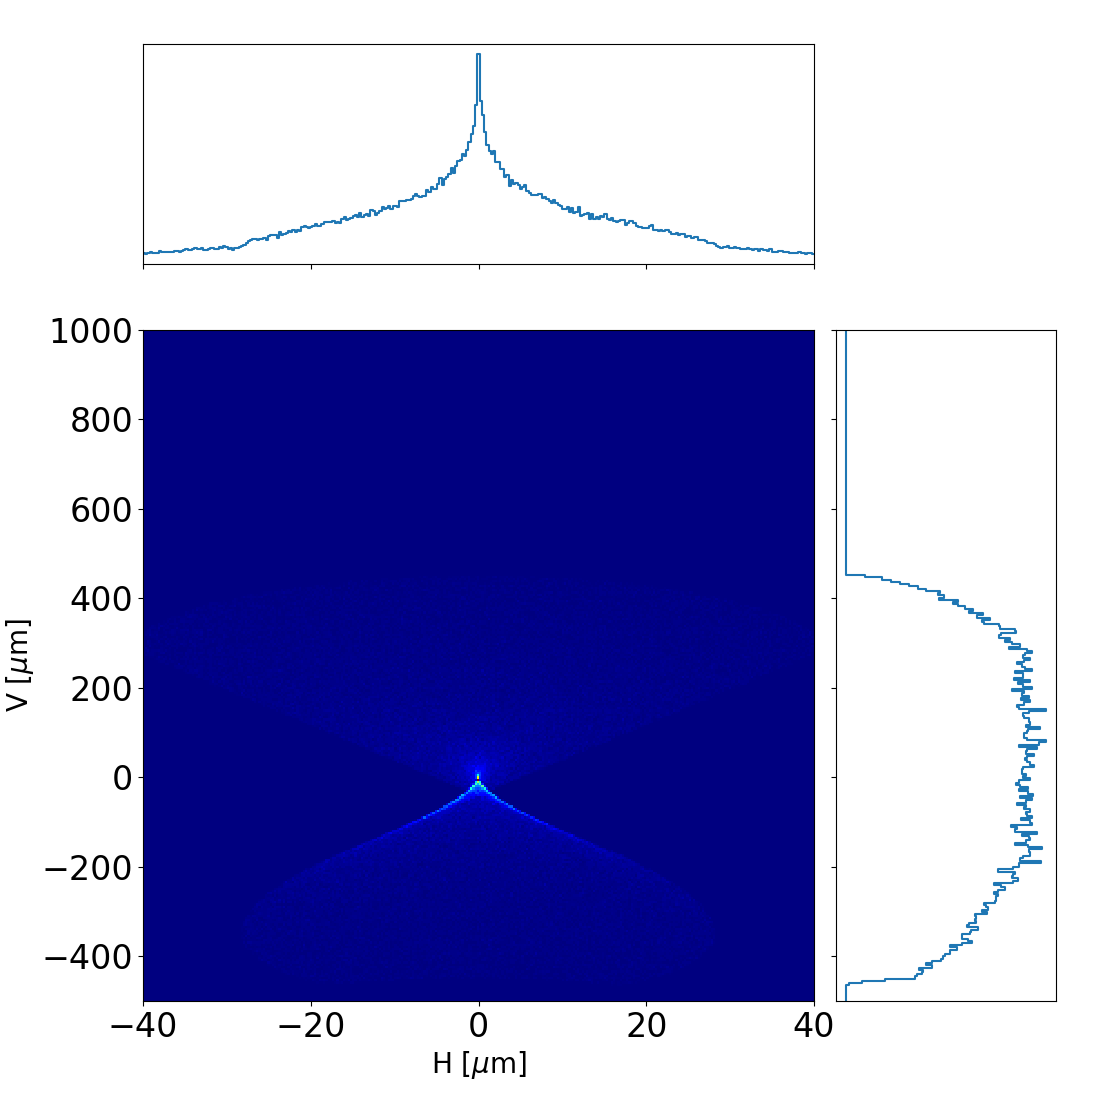
\includegraphics[width=0.22\textwidth]{figures/p2s_toroid_z.png}
\caption{\label{fig:pointToSegment}Comparison of images produced by different surfaces. From left to right: a) Diaboloid (Eq.~\ref{eqn:diaboloidV}), b) Diaboloid (Eq.~\ref{eqn:diaboloidK}), c) parabolic-cone (Eq.~\ref{eqn:parabolicCone}) and d) toroid (Eq.~\ref{eqn:toroid}). In the second raw, the same images but with the horizontal scale zoomed to observe the residuals: for the diaboloid the Full-Width at Half-Maximum (FWHM) is 88 nm in both cases (Eq.~\ref{eqn:diaboloidK} and Eq.~\ref{eqn:diaboloidV}), 22 nm for the parabolic-cone, and 2.5 $\mu$m for the toroid (note the different scale for this one).
}
\end{figure}

The expected result at the focal position is a line focus (segment) with zero dimension in horizontal and a length of $L\sin\theta$ in vertical. The ray-tracing results are shown in Fig.~\ref{fig:pointToSegment} where the focal images for different surfaces are compared: DiaboloidV (Eq.~\ref{eqn:diaboloidV}), DiaboloidK (using Eq.~\ref{eqn:diaboloidK}), parabolic-cone (Eq.~\ref{eqn:parabolicCone}) and Toroid (Eq.~\ref{eqn:toroid}). The results (top figures) show that all the surfaces produce a line focus, which is very narrow for the Diaboloid. The approximated surfaces (parabolic-cone and toroid) show some width, evidencing the benefit of using the Diaboloid. The intensity profile along the vertical direction has a non-uniform profile due to the fact that the beam has not a uniform distribution when projected on the mirror surface with a grazing angle. Indeed, not all the mirror is illuminated, and the upper angles of the mirror are shadowed by the beam. 



To study the aberrations produced by the different surfaces analyze in detail the width at the focal position. It should be zero for the Diaboloid (by definition), but some "residual" width is expected. This can be appreciated in the bottom raw of Fig.~\ref{fig:pointToSegment}. The residual width for the Diaboloid may be related to several factors discussed in the next paragraphs: i) truncation errors in the numerical simulations, ii) errors due to the limited number of sampling points, iii) errors due to the use of the "basal plane approximation" to rotate the Diaboloid from the canonical-mirror system to the mirror-related coordinates (as discussed in Section~\ref{sec:DiaboloidEqs}), and iv) errors inherent to the ray tracing implementation. 

\begin{figure}[h]
\flushleft
~~~~~~a)~~~~~~~~~~~~~~~~~~~~~~~~~~~~~~~~~~~~~~~~~~~~~~~~~~~~~~~~~~~~b)\\
\centering
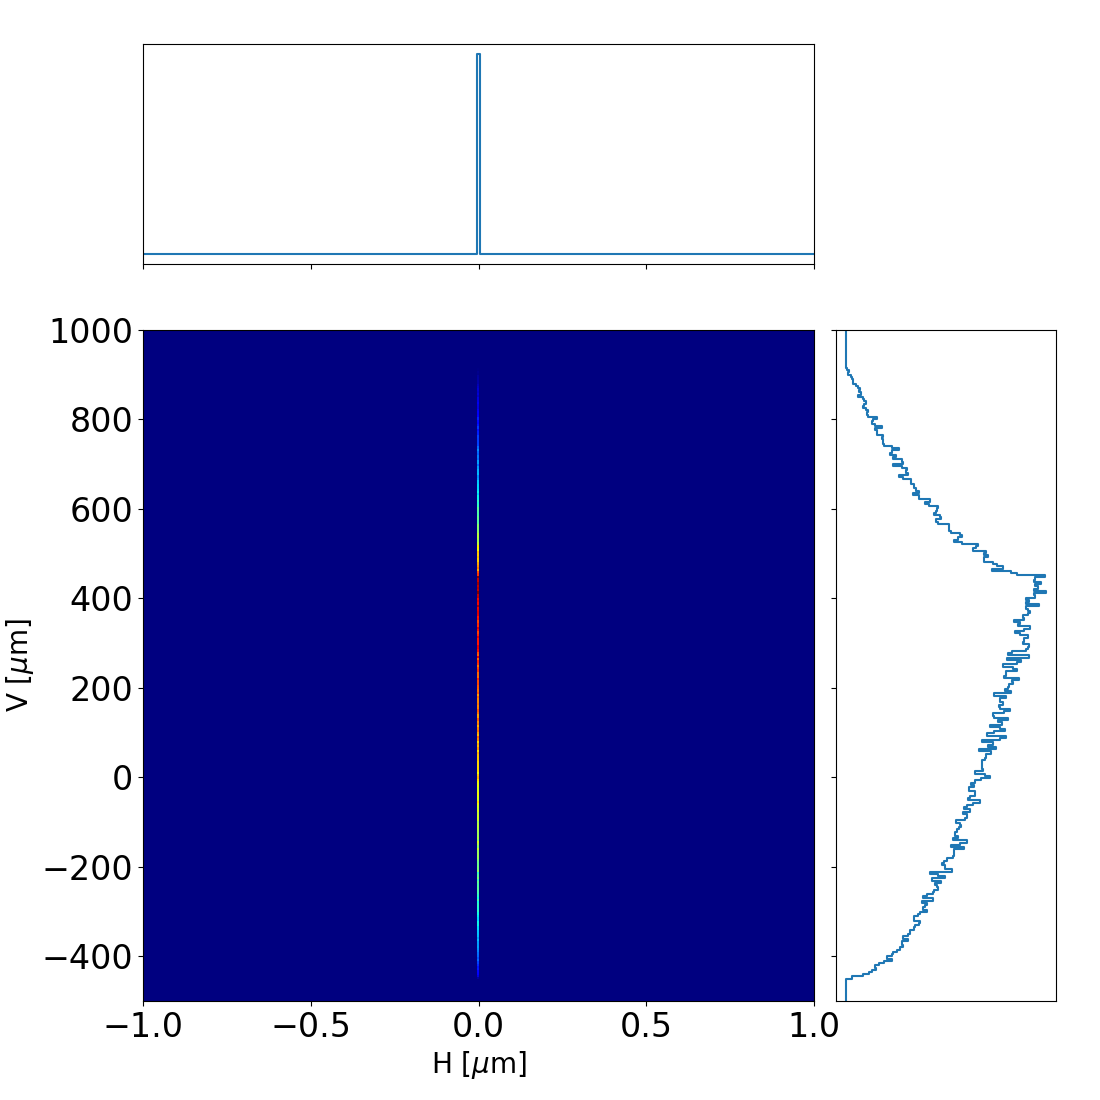
\includegraphics[width=0.35\textwidth]{figures/p2s_mathematica1.png}
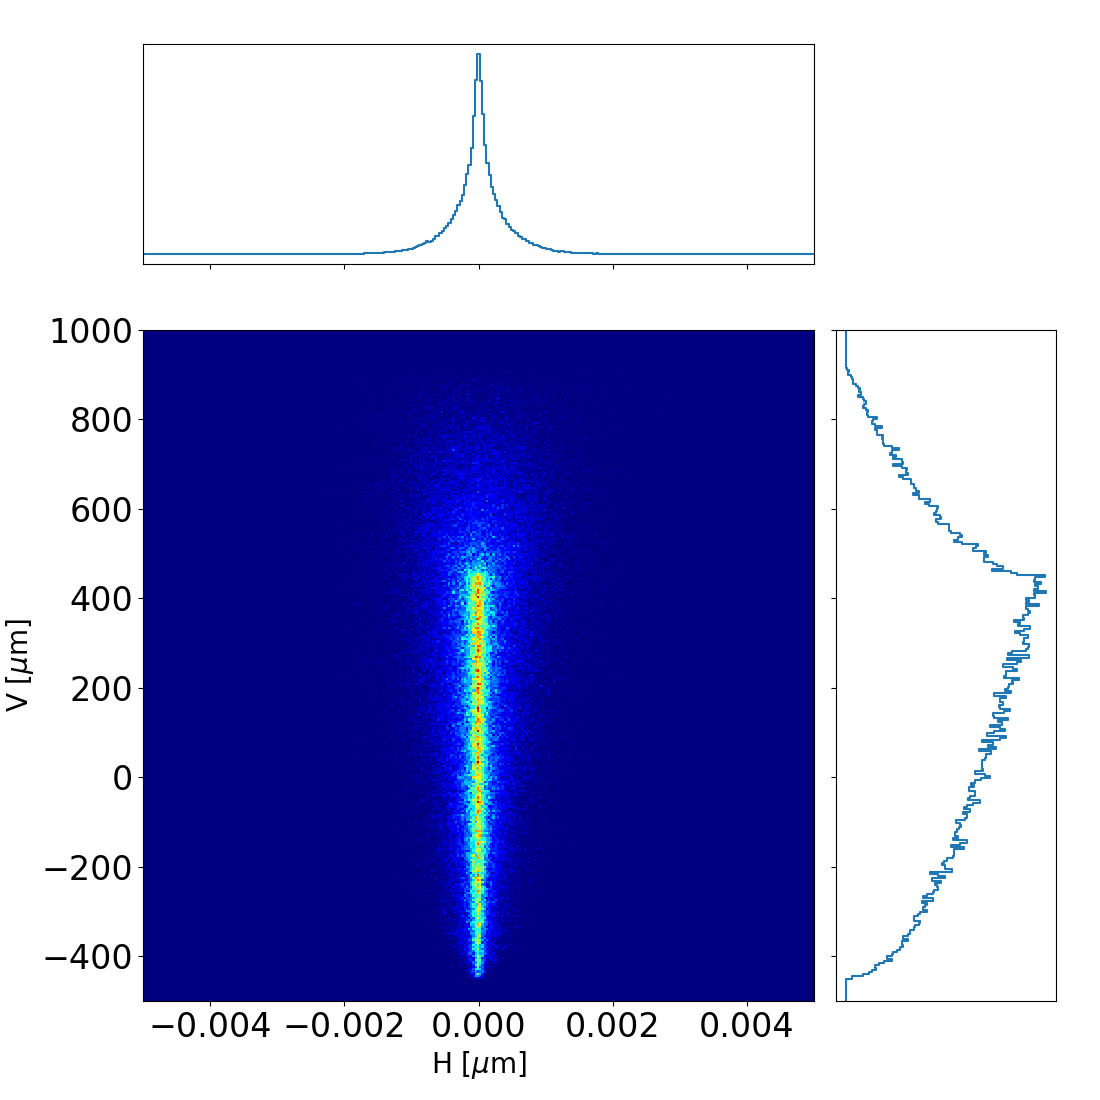
\includegraphics[width=0.35\textwidth]{figures/p2s_matematica2.png}
\caption{\label{fig:mathematica}Focal image produced by a Diaboloid calculated using the exact rotation (see text). The graphics show two different horizontal scale: a) to compare with Figs.~\ref{fig:pointToSegment}a,b, and b) zoomed to resolve residual structure width (0.2 nm).
}
\end{figure}


%Then we propagated one meter downstream the focal line and a rectangle is produced, as we go out of focus in horizontal but in vertical the beam is collimated thus keeping the same length than in the focal position.

 
The expected numeric rounding errors are small. The surface evaluation and ray tracing simulations are performed in double precision. The surface is passed from the "Diaboloid widget" to the SHADOW engine via files (one {\tt hdf5} and its translation into SHADOW surface) but the numbers are written in "scientific format". The precision (rounding error) or machine epsilon\footnote{ https://en.wikipedia.org/wiki/Machine\_epsilon} in double precision floating arithmetic is of the order of 2.2 $\times$ 10$^{-16}$. If we work with length units in meters, that corresponds to to less than one femto-second, therefore for our practical purposes, where we work maximum to nano-focusing, this is not a limiting issue. Typically we will use number of points for the $X$ and $Y$ axes in the order of 100-10000 (for our simulations we used 1001 in $Y$ and 101 in $X$). The possible error can be checked by modifying it. With 1001 $\times$ 101 points we get a residual width of 88 nm for the Diaboloid, and 79 nm if the number of points in the axes is two times and 33 nm is is four times. This is due to the interpolation that the ray-tracing does using the polynomial spline. A surface with "enough" points should be used, being limited by the maximum acceptance of SHADOW (500 points in $X$, unlimited in $Y$). 

The "basal-plane-approximation" is a critical issue. We can compare the residuals in width for the Diaboloid calculated with the method described here using the "basal plane-approximation" (88 nm) with a surface produced following the exactly rotated Diaboloid surface \cite{Valeriy2020b} implemented in Mathematica \cite{lacey}  (Fig.~\ref{fig:mathematica}) that gives 0.2 nm width. There is therefore an significant increase of the residual due to the use of "basal-plane-approximation". However, even using this approximation, the residual width is small enough to allow performing simulations with the goal of comparing the optical performances of the Diaboloid and compare it with with other surfaces. As commented before, the calculation of the numeric mesh with the exactly rotated surface (\cite{Valeriy2020b}) is possible, but has to be done with Mathematica outside the Oasys environment thus making more time consuming the simulations.  A last comment is regarding the ray-tracing procedure to compute the intersection of the rays with a surface that is numerically defined. It uses an iterative approximation to get to the "correct" interaction point, and there is an intrinsic error there. From our experience with SHADOW, this has never been a limiting factor, and we do not expect it here as the surfaces are smooth. To check this fact we have compared  Diaboloid ray-tracing in two ways, first the usual way to add the numeric mesh on top of a plane mirror, and second to add the Diaboloid with a toroid removed on top of a SHADOW Toroid. The heights in the numeric mesh for the second case are smaller thus we expect smaller errors. We obtained, however, the opposite result: 95 nm for the Diaboloid detrended with a toroid (vs 88 nm for the undetrended case). As a practical conclusion, it is better to use the Diaboloid mesh on top of a plane mirror in SHADOW.

After the analysis of all possible sources of error, we can conclude that small errors are due to numerical round errors, sampling points and iterative algorithms to find ray intersects. They contributed to about 0.2 nm in the focal spot (Fig.~\ref{fig:mathematica}a). There is a more important error due to the basal-plane approximation used in the Diaboloid widget in Oasys (88 nm, Fig.~\ref{fig:pointToSegment}a,b). However, these errors are in the sub-micron level. Therefore we could can accept this approximation for studying the Diaboloid surface and compare with other approximated surfaces when the differences are at the level of what is optically detectable in experiments (larger than about 0.1$\mu$m).

\section{Ray-tracing of an existing beamline}
\label{sec:beamline}

In this section we analyze the possible use of a Diaboloid in a real beamline. We study the case of beamline 12.2.2  at ALS \cite{bl1222} \cite{MacDowell2004}. The source of this beamline is a bending magnet. We consider three cases: i) using a source point, ii) the ALS ring
$\sigma_x$ = 26 $\mu$m, $\sigma_y$ = 10 $\mu$m, ring electron energy $E_e$=1.9 GeV, magnetic field $B$=5.28~T, photon energy $E$=30 keV, and ii) the ALS-U ring, with $\sigma_x$ = 10 $\mu$m, $\sigma_y$ = 7 $\mu$m, $E_e$=2.0~GeV, $B$=3.1~T, $E$=30~keV. We study the two beamline mirrors: M1 a plane parabola, at $p_1$=6.5~m from the source ($L$ = 900~mm, $\theta$=2 ~mrad) and M2 a toroid/diabolod/parabolic-cone in a Type II (segment-to-point) configuration at $p_2$=18.8~m from the source ($L$=800~mm, $W$=20~mm, $\theta$ = 2~mrad. The exit slit (focal plane) is at $D$=26.875~m from the source.  The M2 magnification M= $(D-p_2)/p_2$=0.43 is close but not exactly matching the "golden" 1:2 toroid geometry \cite{padmore2000, howells2000}. This beamline uses M1 to collimate the beam in the vertical direction in order to optimize the monochromator performance (not simulated) and then M2 refocus the beam at the entrance slit, therefre M2 sees the source at infinity in vertical and at $p_2$ in horizontal. The possible use of a diaboloid or a parabolic-cone mirror in M2 is studied and the performances compared with the current solution (toroid).

\begin{figure}[h]
\flushleft
a)~~~~~~~~~~~~~~~~~~~~~~~~~~~~~~~~~~~b)~~~~~~~~~~~~~~~~~~~~~~~~~~~~~~~c)~~~~~~~~~~~~~~~~~~~~~~~~~~~d)\\
\centering
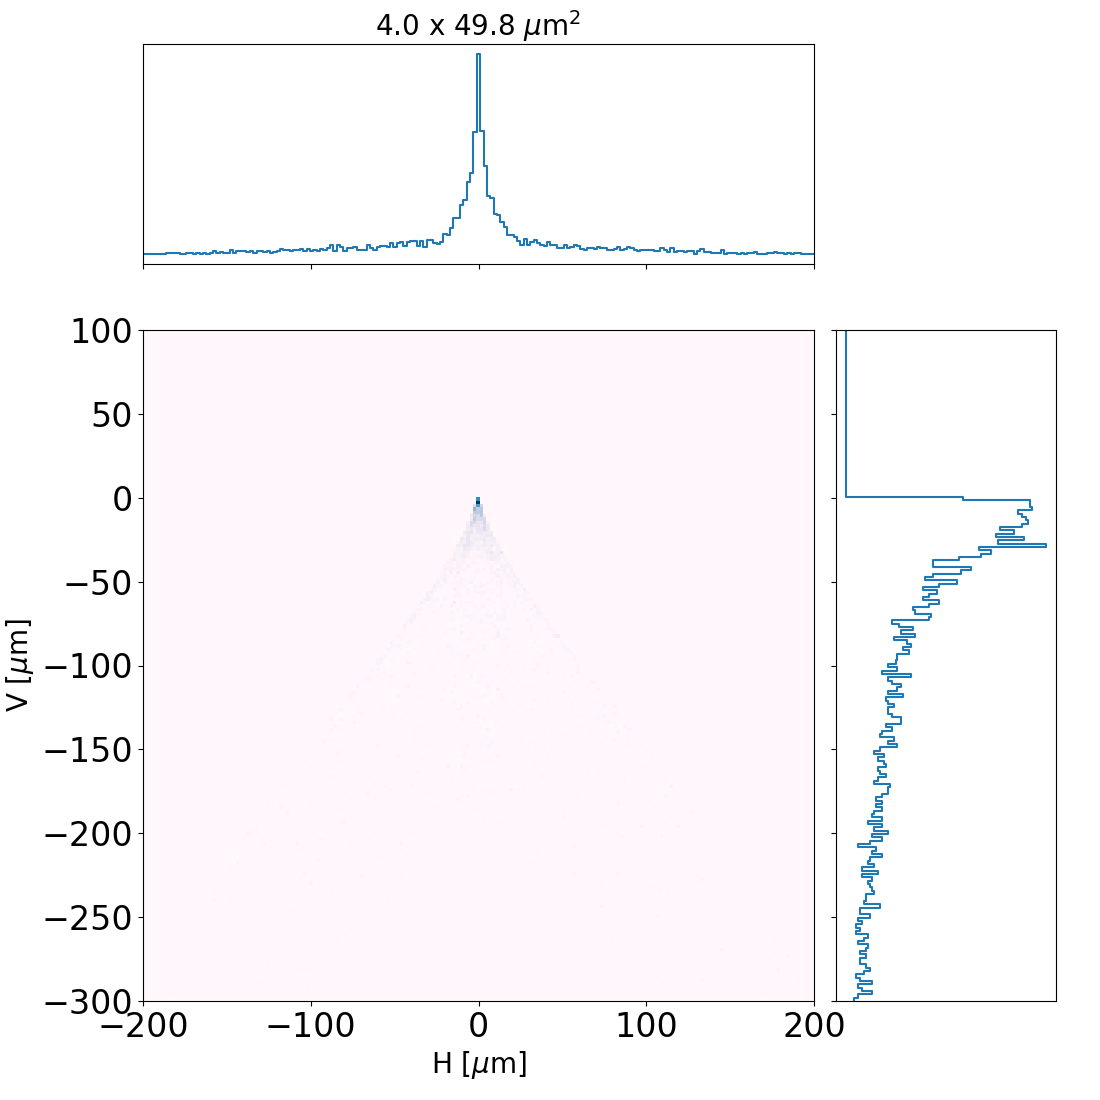
\includegraphics[width=0.24\textwidth]{figures/bl_point_toroid.png}
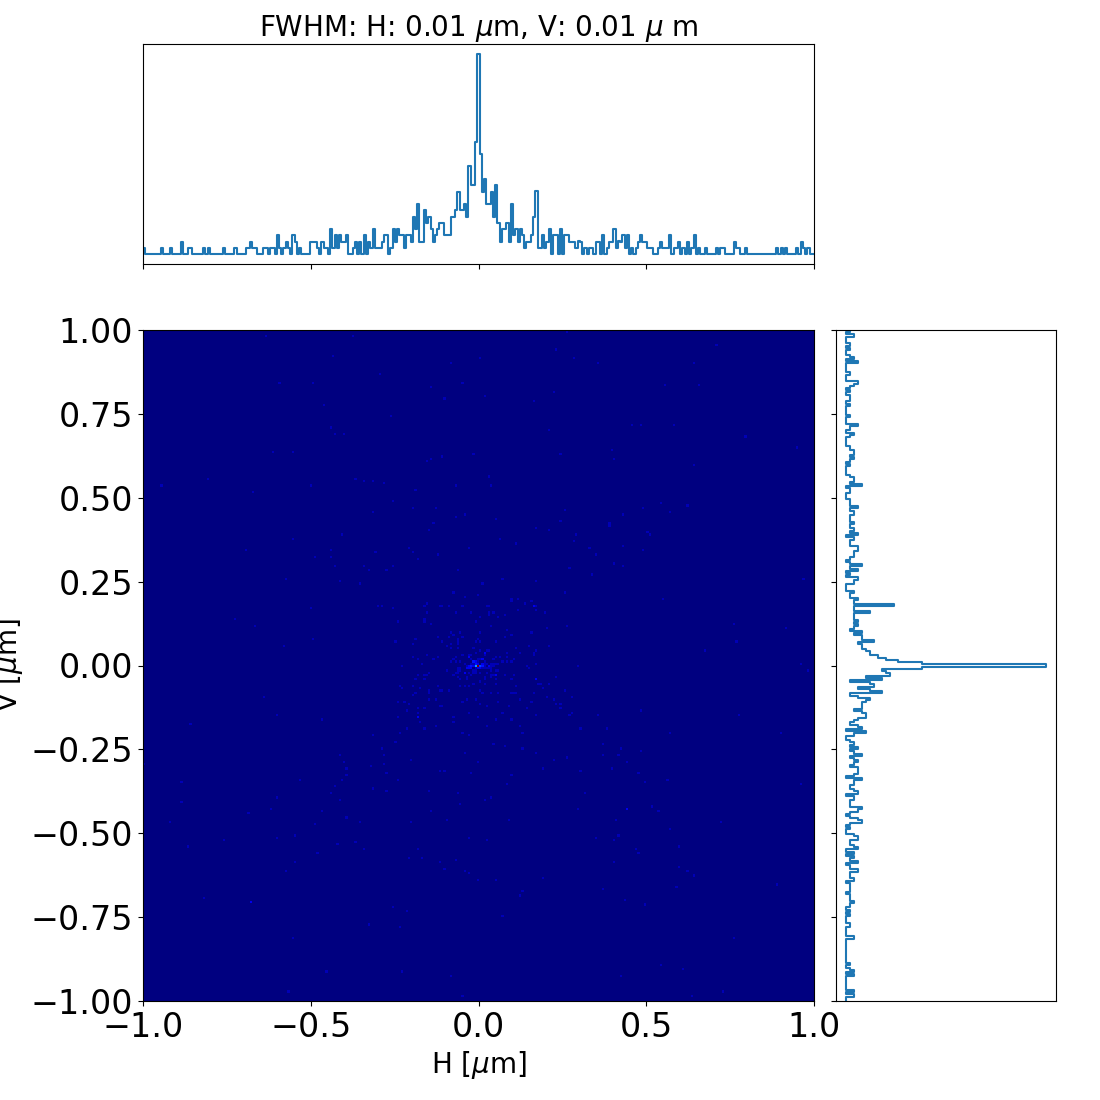
\includegraphics[width=0.24\textwidth]{figures/bl_point_parabolic-cone.png}
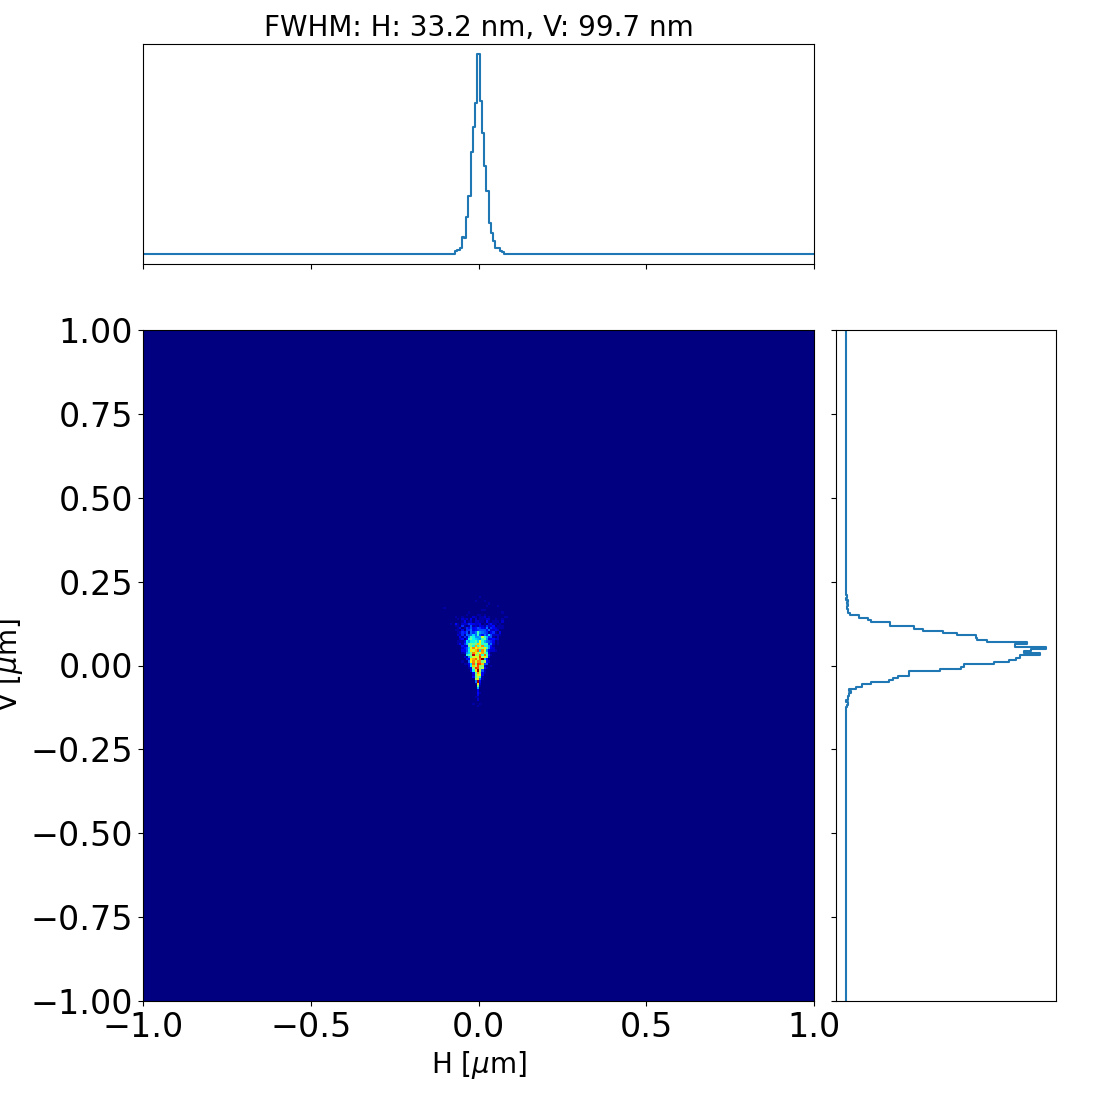
\includegraphics[width=0.24\textwidth]{figures/bl_point_diaboloid.png}
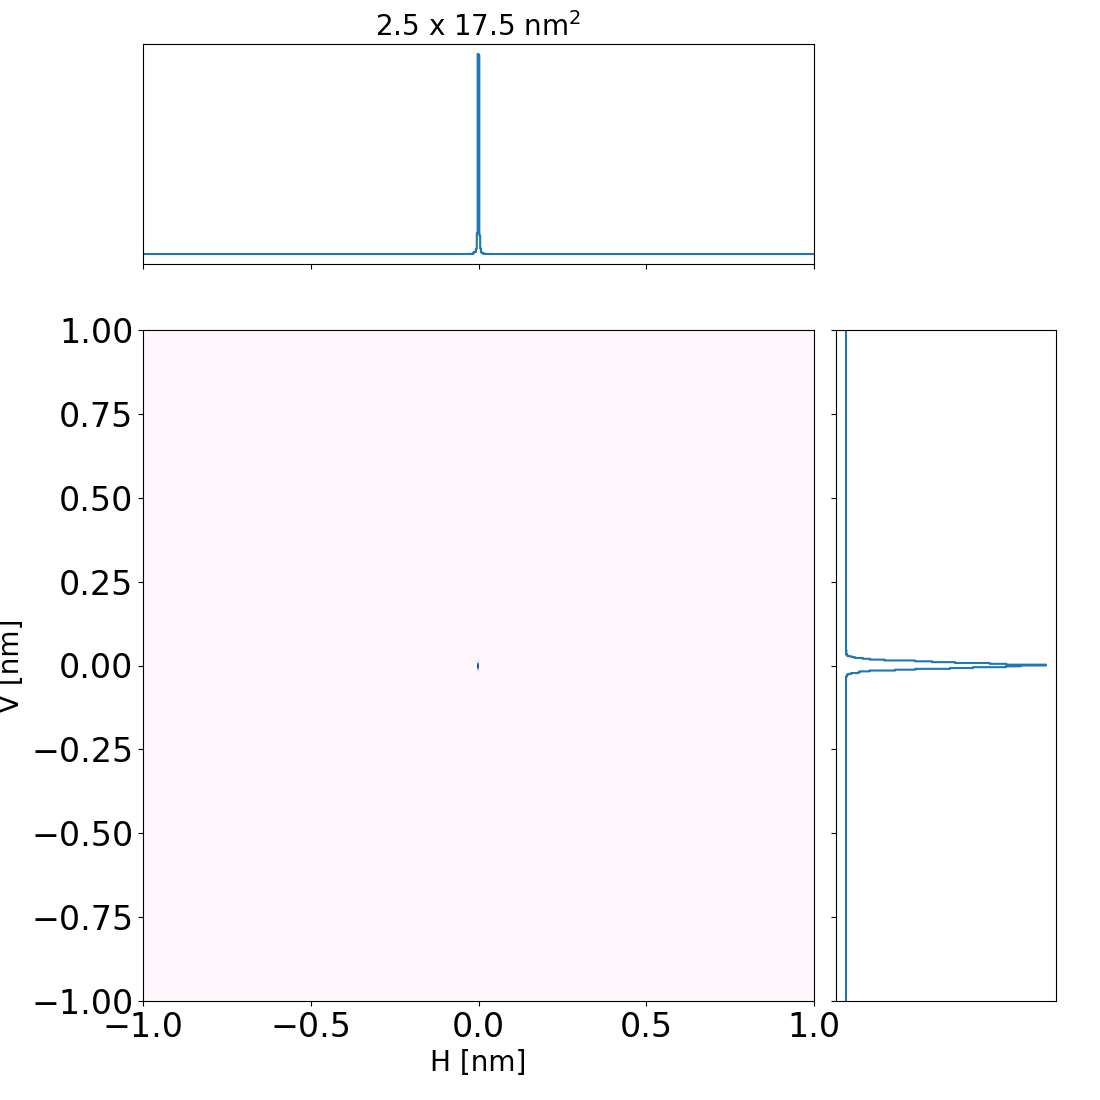
\includegraphics[width=0.24\textwidth]{figures/bl_point_diaboloid-exact.png}
\caption{\label{fig:bl}Focal image produced by a system of two mirrors M1 (collimating parabola) and M2 represented by (a) a toroid, (b) a parabolic-cone, (c) a Diaboloid using the "basal-plane approximation", and d) a Diaboloid implemented with the exact rotations using code in Ref.~\cite{lacey}. The FWHM of the horizontal and vertical histograms are given in the plot titles. The scale changes in the different plots. Note the large size given by the toroid (4 $\times$ 50 $\mu$m$^2$) contrary to all the other surfaces (submicron level)
}
\end{figure}

Figure~\ref{fig:bl} shows a source point imaged by the beamline using for M2 a toroid, a parabolic-cone and a Diaboloid. The Diaboloid is computed using both the "basal-plane approximation" as implemented in Oasys, and also the exact shape produced by the Mathematica code \cite{lacey}. The use of a point source helps to address the residual widths for the Diaboloid, because it should give zero width. As discussed in the previous section, numeric and sampling errors (due to round errors and iterative calculations of the intercept) produce here a residual of 2.5 $\times$ 17.5 nm$^2$, which is increased to values of 60 $\times$ 32.5 nm$^2$ when using the "basal-plane approximation". In both cases they are at the sub-micron level therefore negligeable with respect to the other effects we want to compare with (source size and aberrations in toroids and parabolic-cones). One can appreciate the high aberrations of the toroid. Two effects can be observed. The intensity profiles produced by the parabolic-cone mirror have aberrated tails not present in the Diaboloid. The vertical FWHM of the parabolic-cone (25 nm) is slightly smaller than the Diaboloid using the "basal-plane approximation" (32.5 nm) therefore can be used to quantify the errors of due to the basal plane approximation, which are not present in the parabolic-cone nor in the exact Diaboloid implementation. 

\begin{figure}[h]
\flushleft
a)~~~~~~~~~~~~~~~~~~~~~~~~~~~~~~~~~~~~~~~~~~~b)~~~~~~~~~~~~~~~~~~~~~~~~~~~~~~~~~~~~~~~~~~~c)\\
\centering
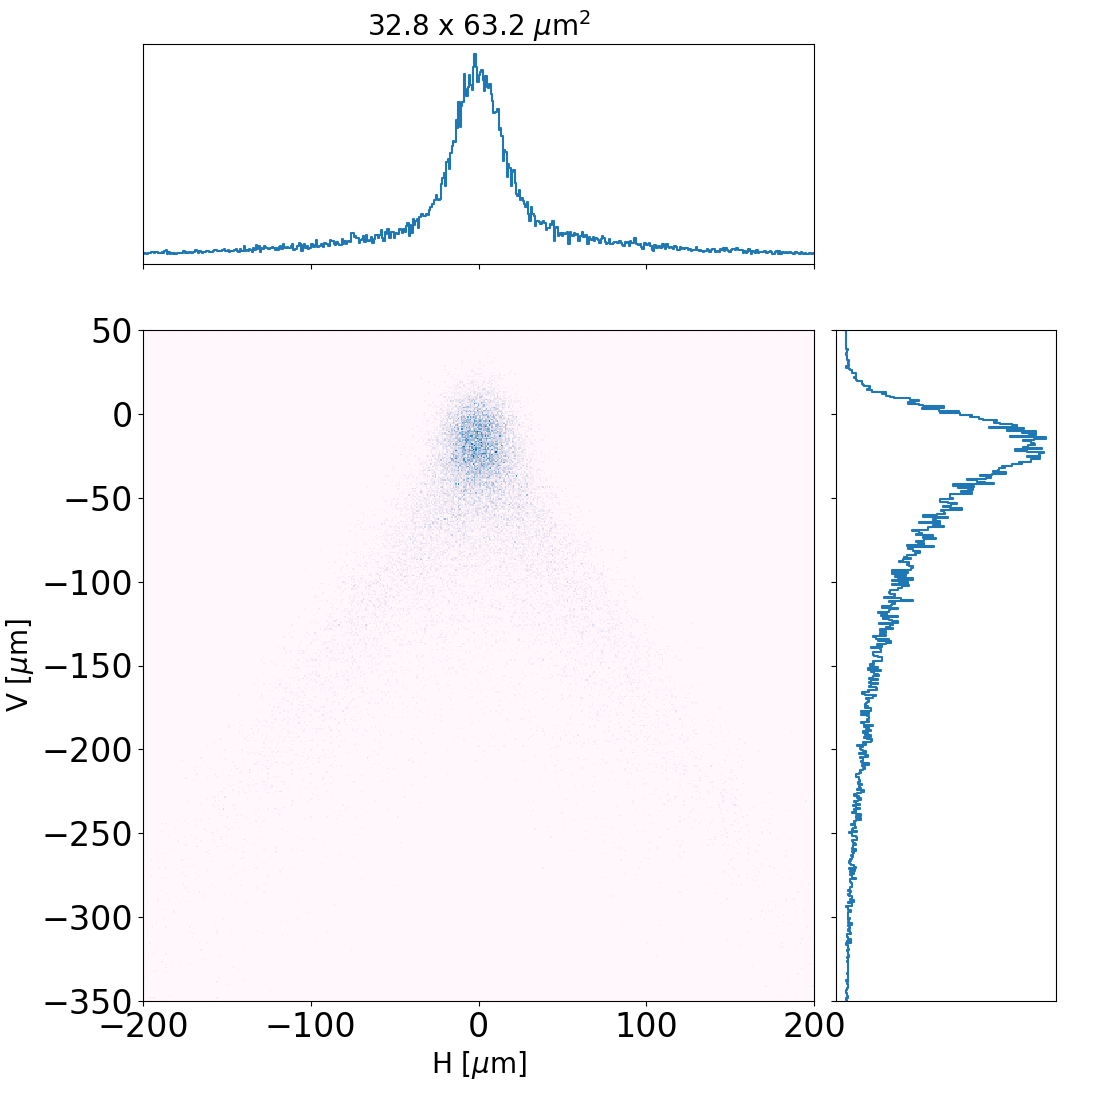
\includegraphics[width=0.32\textwidth]{figures/als_toroid.png}
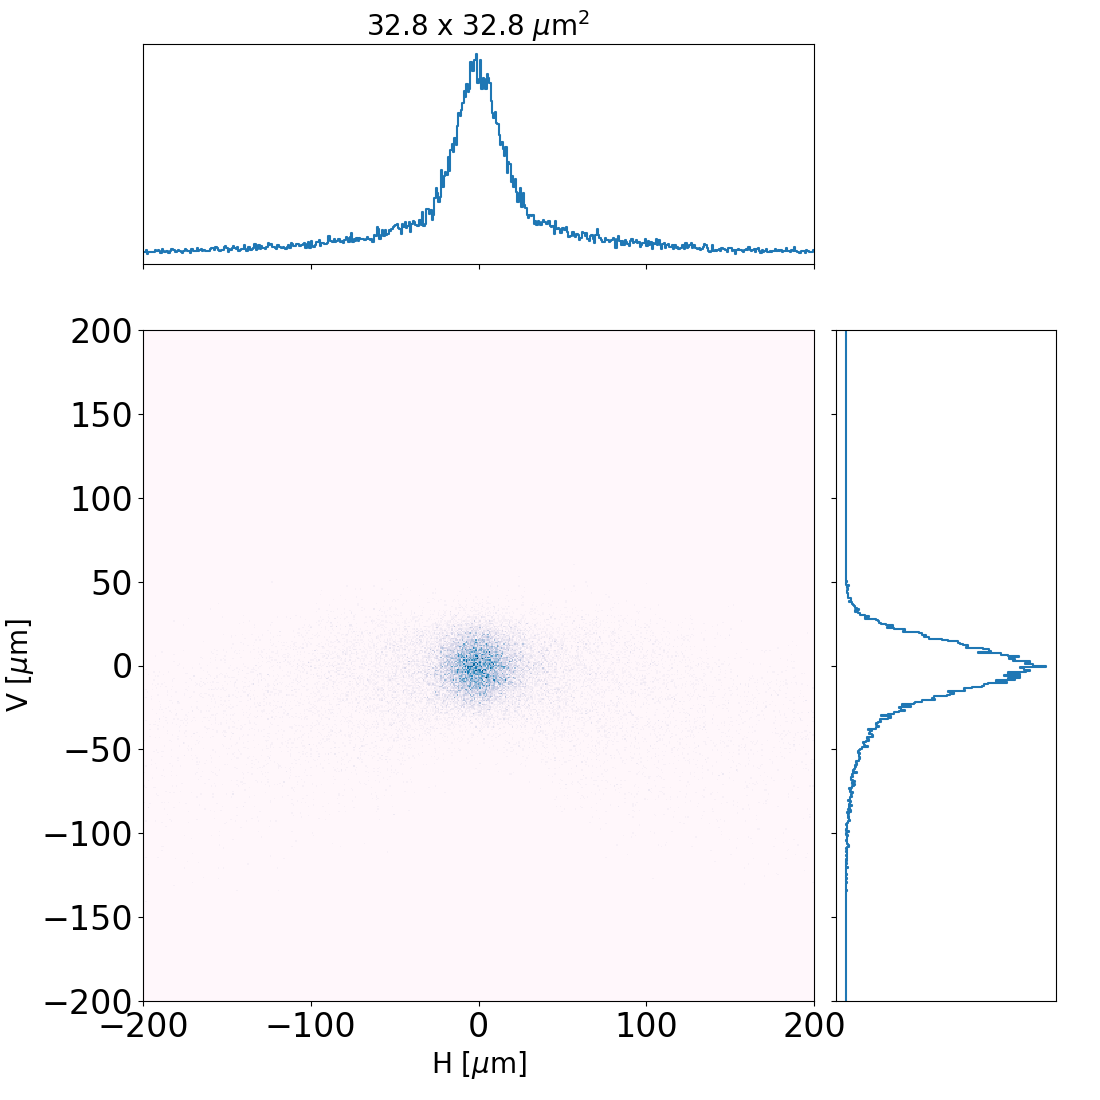
\includegraphics[width=0.32\textwidth]{figures/als_parabolic-cone.png}
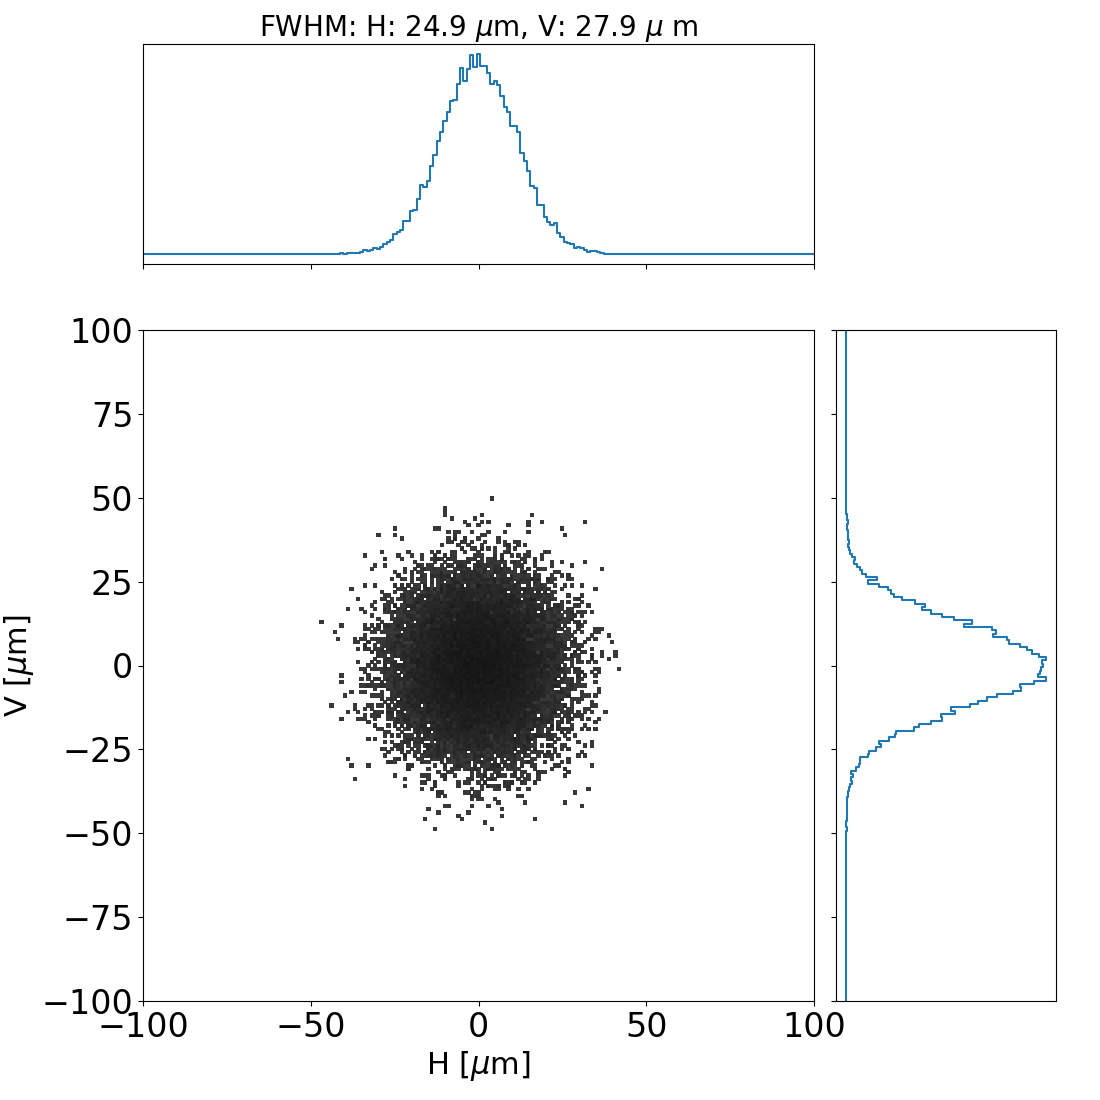
\includegraphics[width=0.32\textwidth]{figures/als_diaboloid.png}

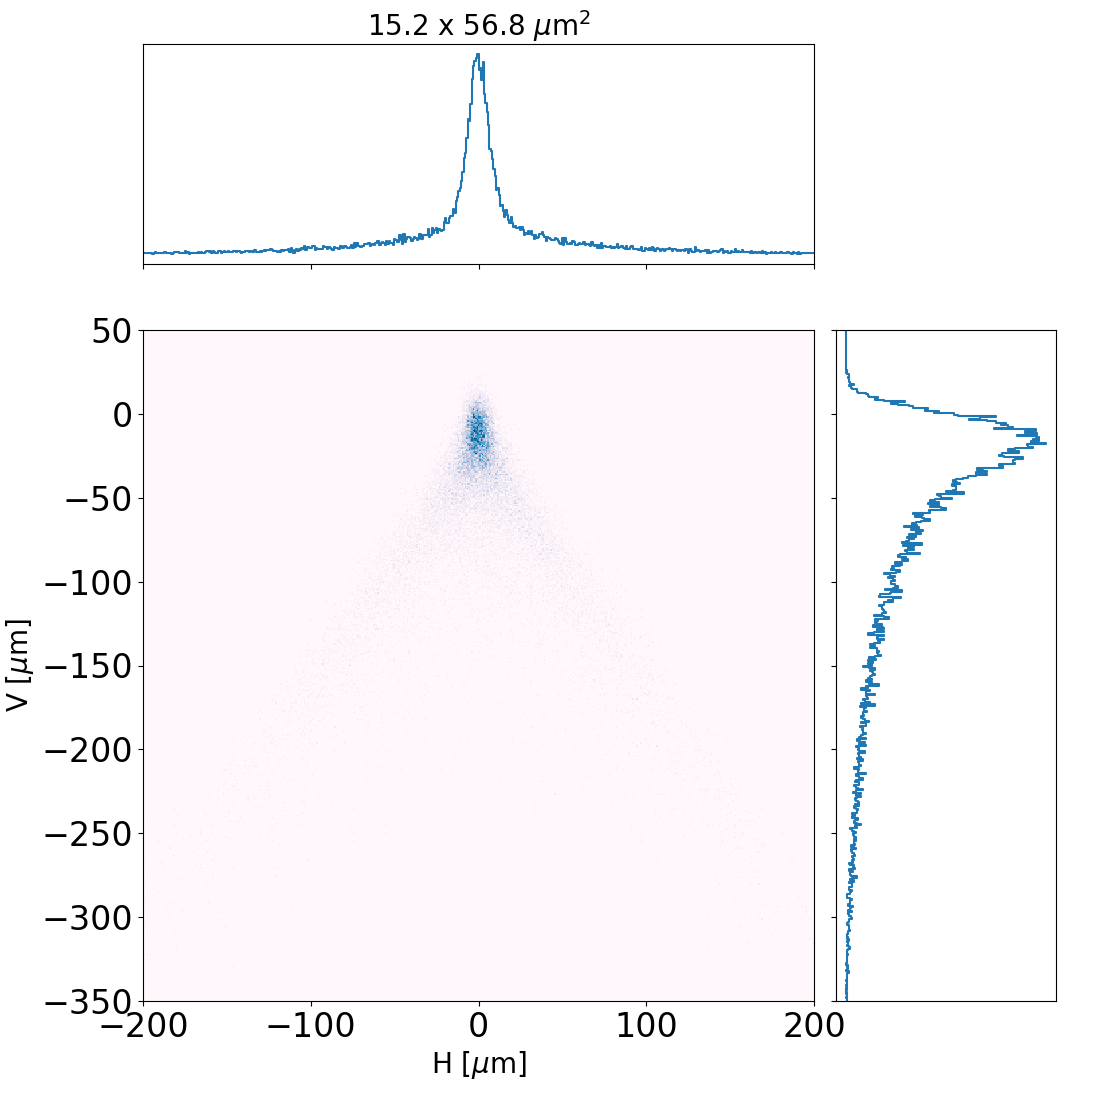
\includegraphics[width=0.32\textwidth]{figures/alsu_toroid.png}
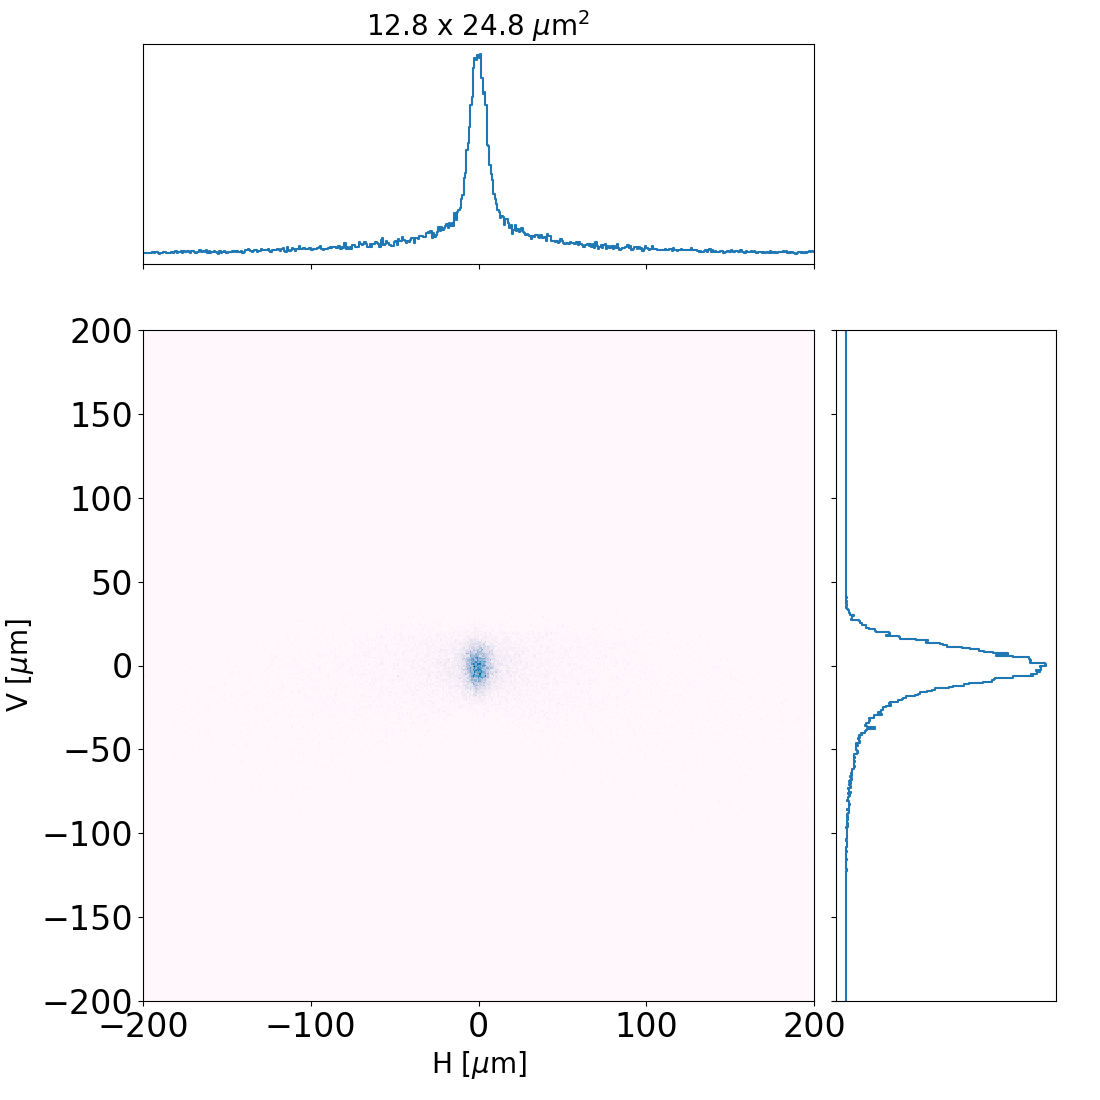
\includegraphics[width=0.32\textwidth]{figures/alsu_parabolic-cone.png}
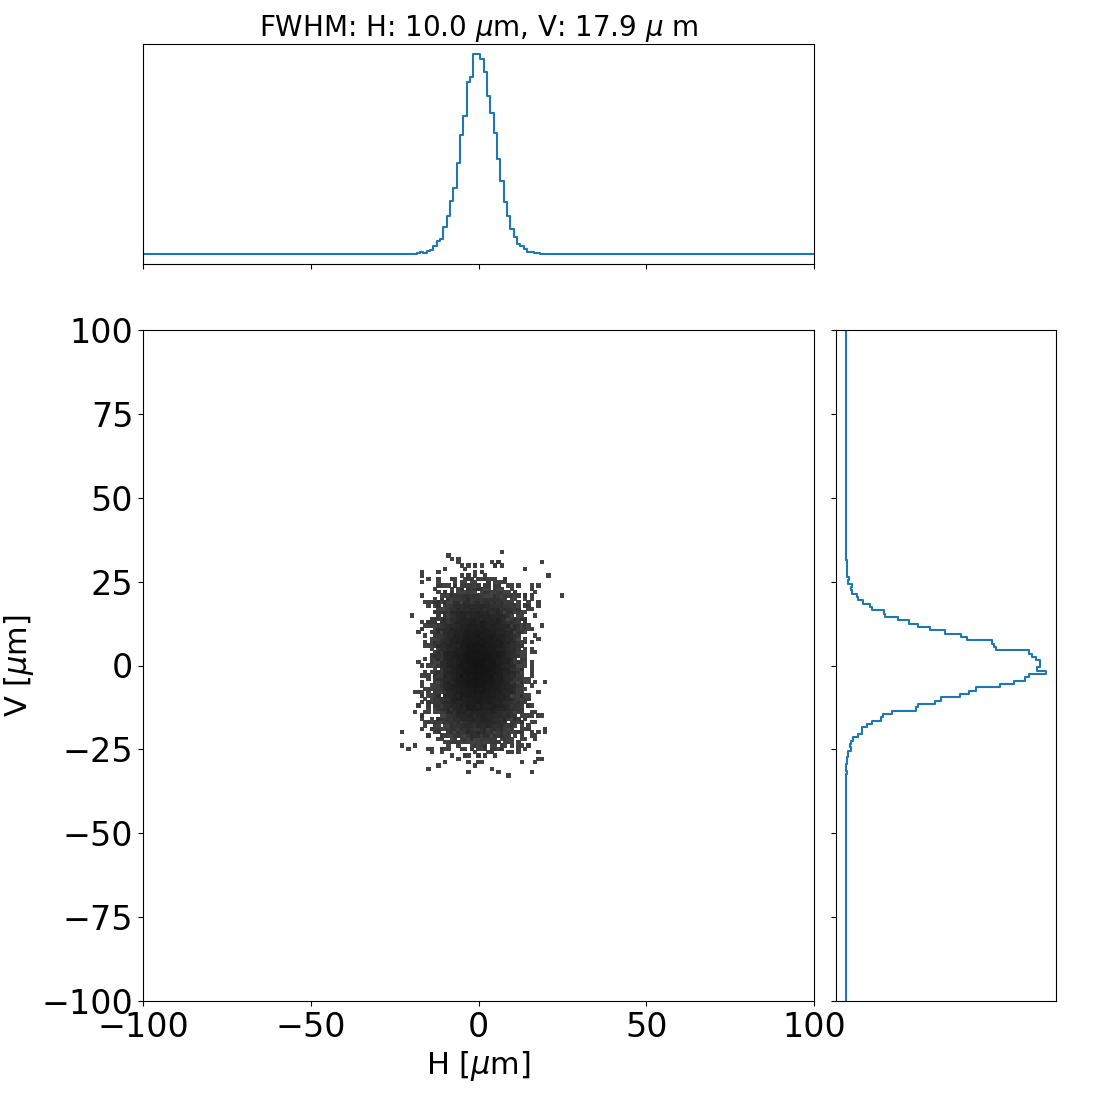
\includegraphics[width=0.32\textwidth]{figures/alsu_diaboloid.png}
\caption{\label{fig:als}Focal image produced by a system of two mirrors M1 (collimating parabola) and M2 represented by a a) toroid, b) parabolic-cone, and c) Diaboloid. The width of the intensity distributions (in FWHM) are written in the graphic titles. 
}
\end{figure}

In Fig.~\ref{fig:als} we compared the images produced by the beamline for a source using the ALS and ALS-U bending magnets. For the ALS case, the Diaboloid obviously improves the Toroid case currently impemented, but the gain is not dramatic: a factor 2 in vertical FWHM and less in horizontal, which justifies the use of toroids because manufacturing Diaboloids is still a challenge. For the ALS-U the gain of using Diabloids is increased to almost a factor 3 in FWHM vertical, which for the toroid is dominated by aberrations. The parabolic-cone is a good approximation as it completely removed the toroid aberrations in vertical, although presenting similar intensity profile in horizontal.

As a conclusion of this section, it is noticeable that for the ALS-U there is a significant improvement in the focal image if the toroid is replaced by a Diaboloid. The parabolic-cone is a good approximation of the Diaboloid, producing an image of comparable with the Diaboloid in terms of FHWM (just a bit larger) but presenting higher tails in the horizontal intensity. 

\section{Comparison of Diaboloid and parabolic-cone for high demagnification}
\label{sec:scan}

In this section we study a possible upgrade of the beamline to obtain a smaller spot size. For that the magnification of the beamline has to be reduced. We study the beamline presented in the last section for ALS-U where the exit arm of the M2 mirror is reduced to have a smaller magnification M=$q/p$. The position of M2 is not changed therefore the length of the beamline is not constant. We have performed ray-tracing simulations where the M factor is changed to values 1:5 and 1:10 (Fig.~\ref{fig:demagnification}). It can be observed the extremely high aberrations produced by the toroid, which makes its use impossible for these configurations. The Diaboloid produces intensity profiles with nice Gaussian profiles, as expected. Interestingly, the parabolic-cone completely removed all the aberration in the toroid presented in the vertical direction producing very good results of beam size FWHM. However, the intensity in horizontal is closer to the toroid than the Diaboloid, with a shape that looks more Lorentzian than Gaussian (higher tails). In vertical the parabolic-cone produces a very clean spot, but not as good as the Diaboloid. 


\begin{figure}[h]
\flushleft
a)~~~~~~~~~~~~~~~~~~~~~~~~~~~~~~~~~~~~~~~~~~~b)~~~~~~~~~~~~~~~~~~~~~~~~~~~~~~~~~~~~~~~~~~~c)\\
\centering
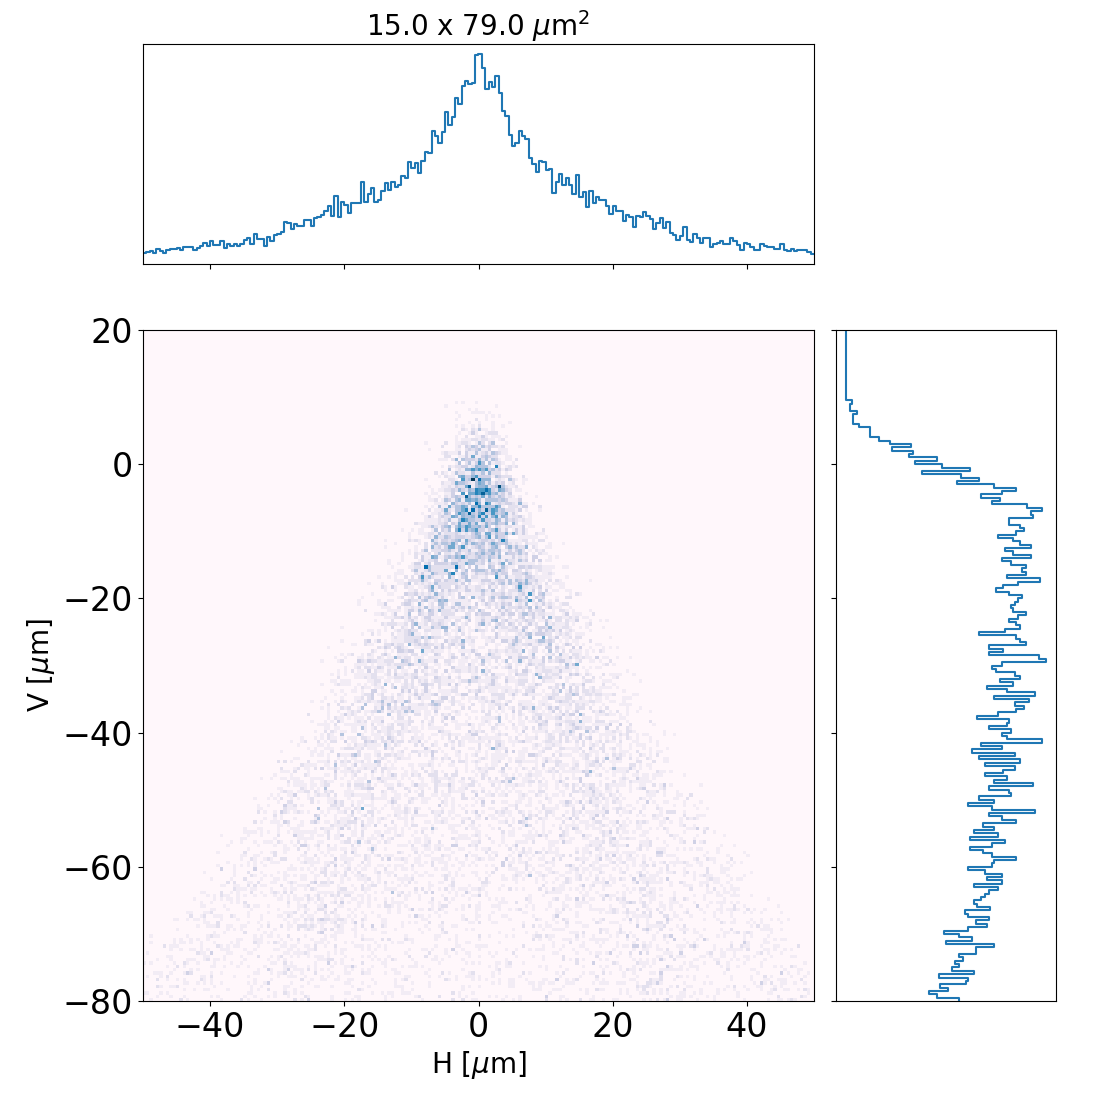
\includegraphics[width=0.32\textwidth]{figures/M0p2_toroid.png}
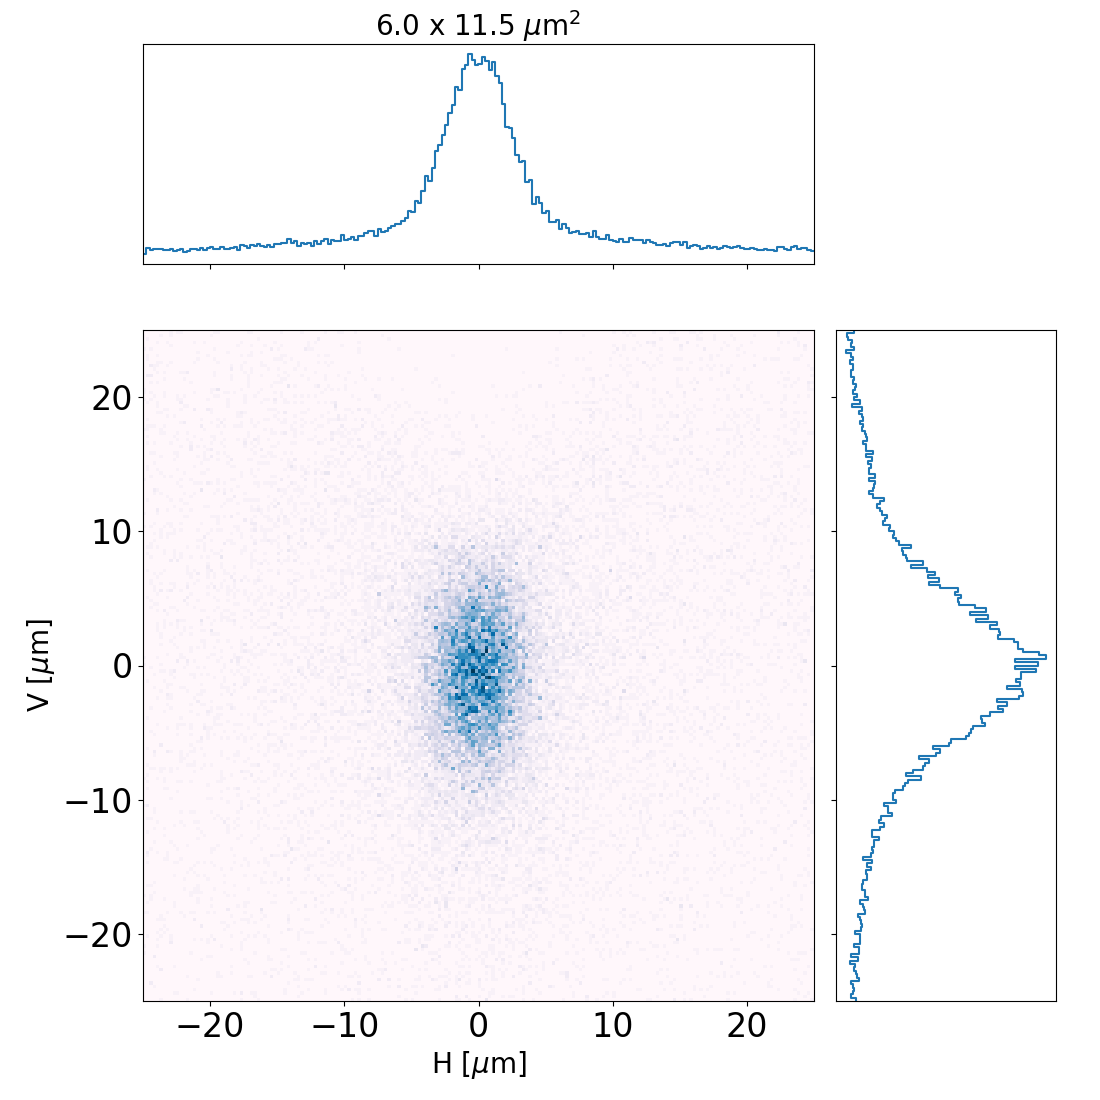
\includegraphics[width=0.32\textwidth]{figures/M0p2_parabolic-cone.png}
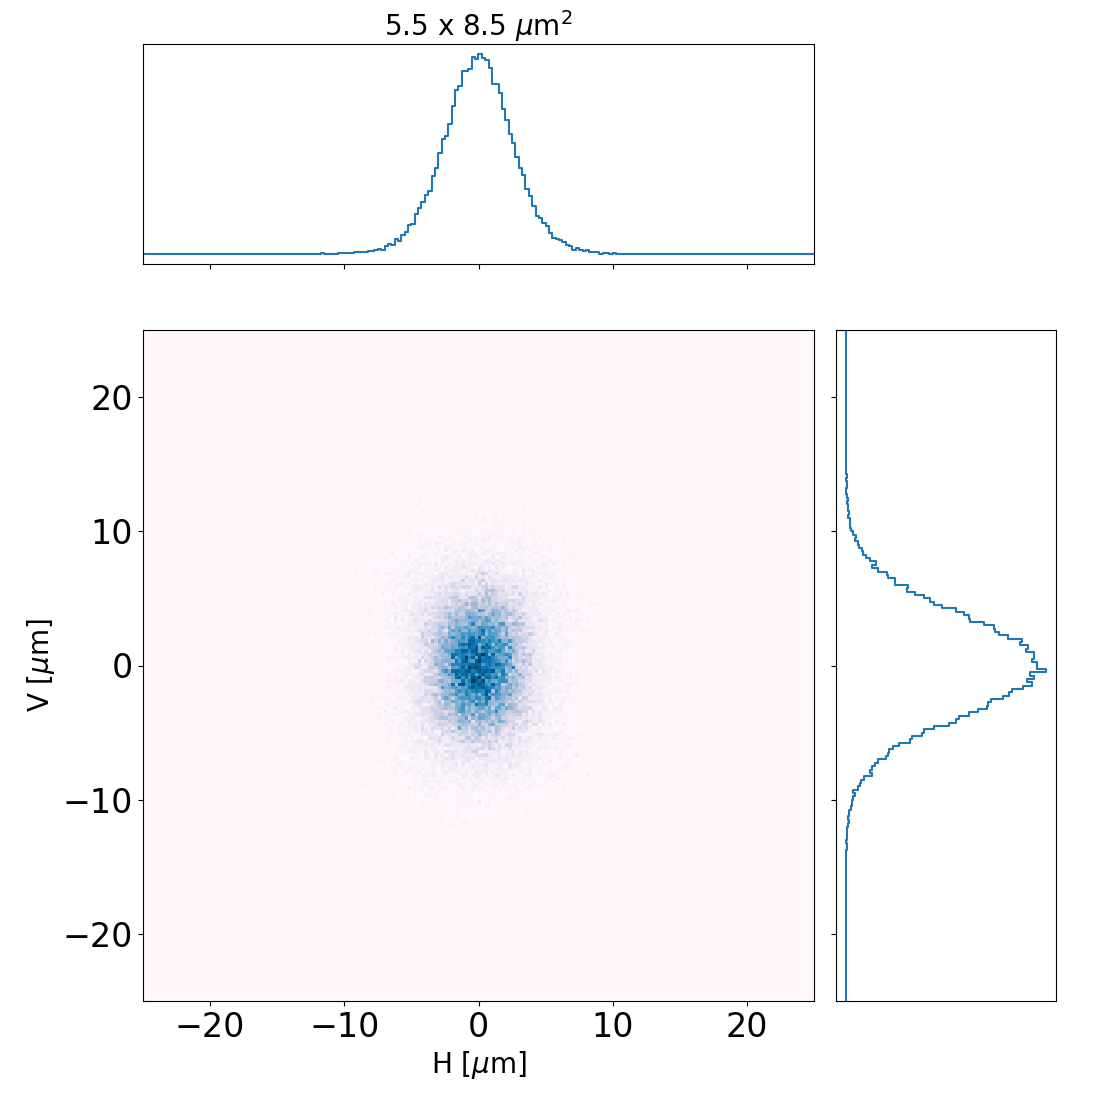
\includegraphics[width=0.32\textwidth]{figures/M0p2_diaboloid.png}
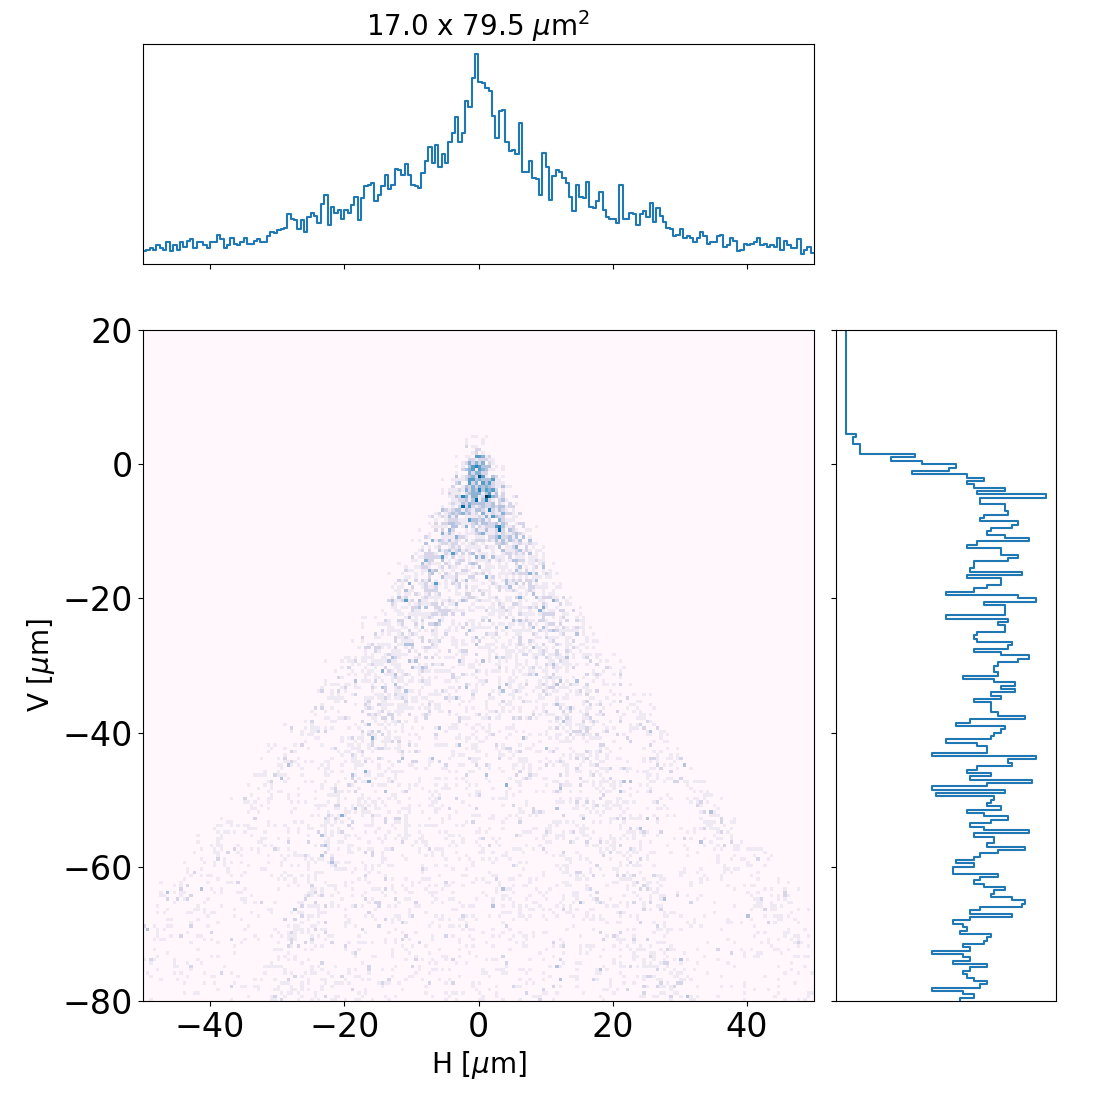
\includegraphics[width=0.32\textwidth]{figures/M0p1_toroid.png}
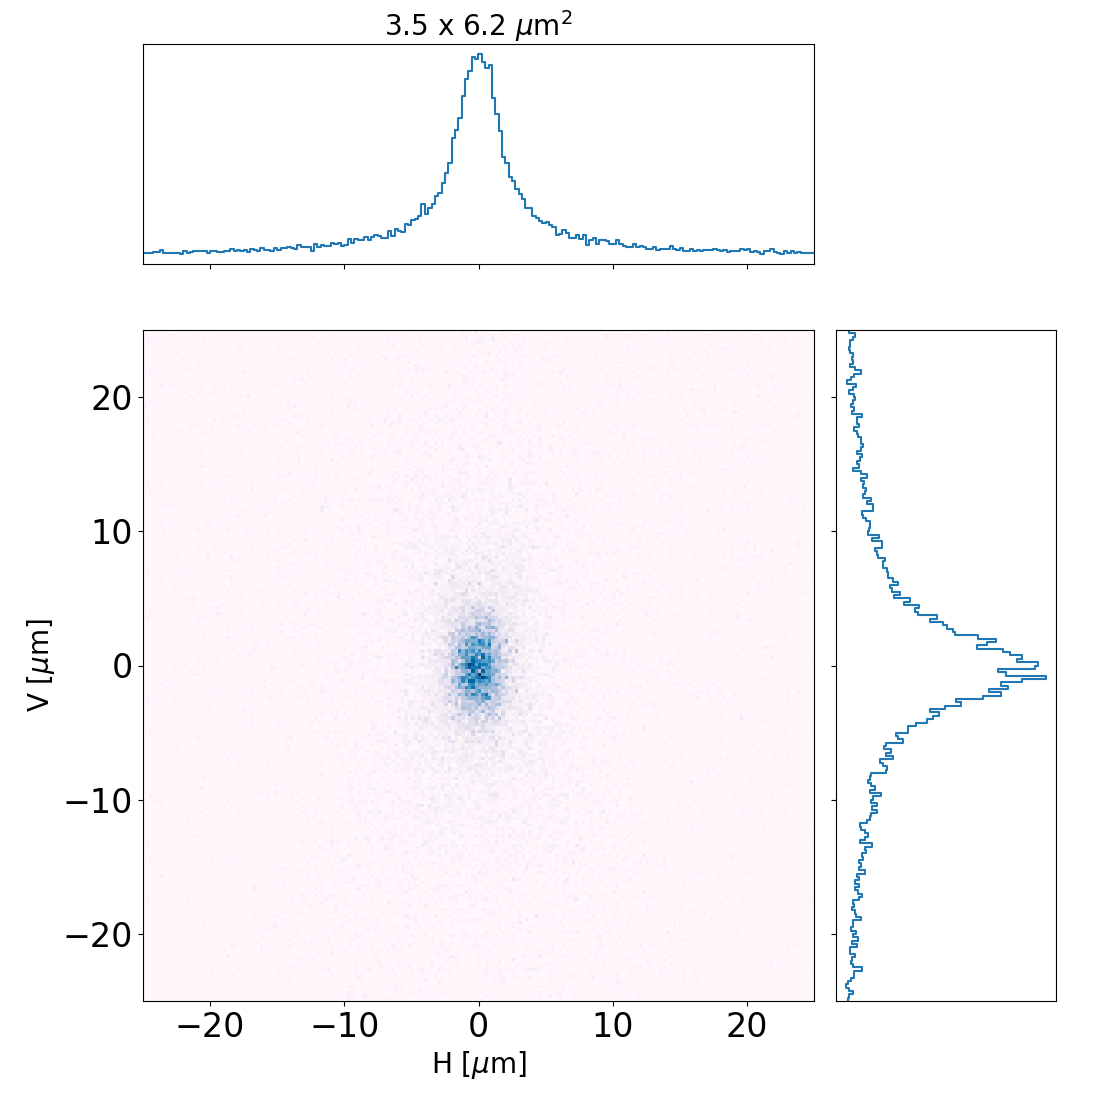
\includegraphics[width=0.32\textwidth]{figures/M0p1_parabolic-cone.png}
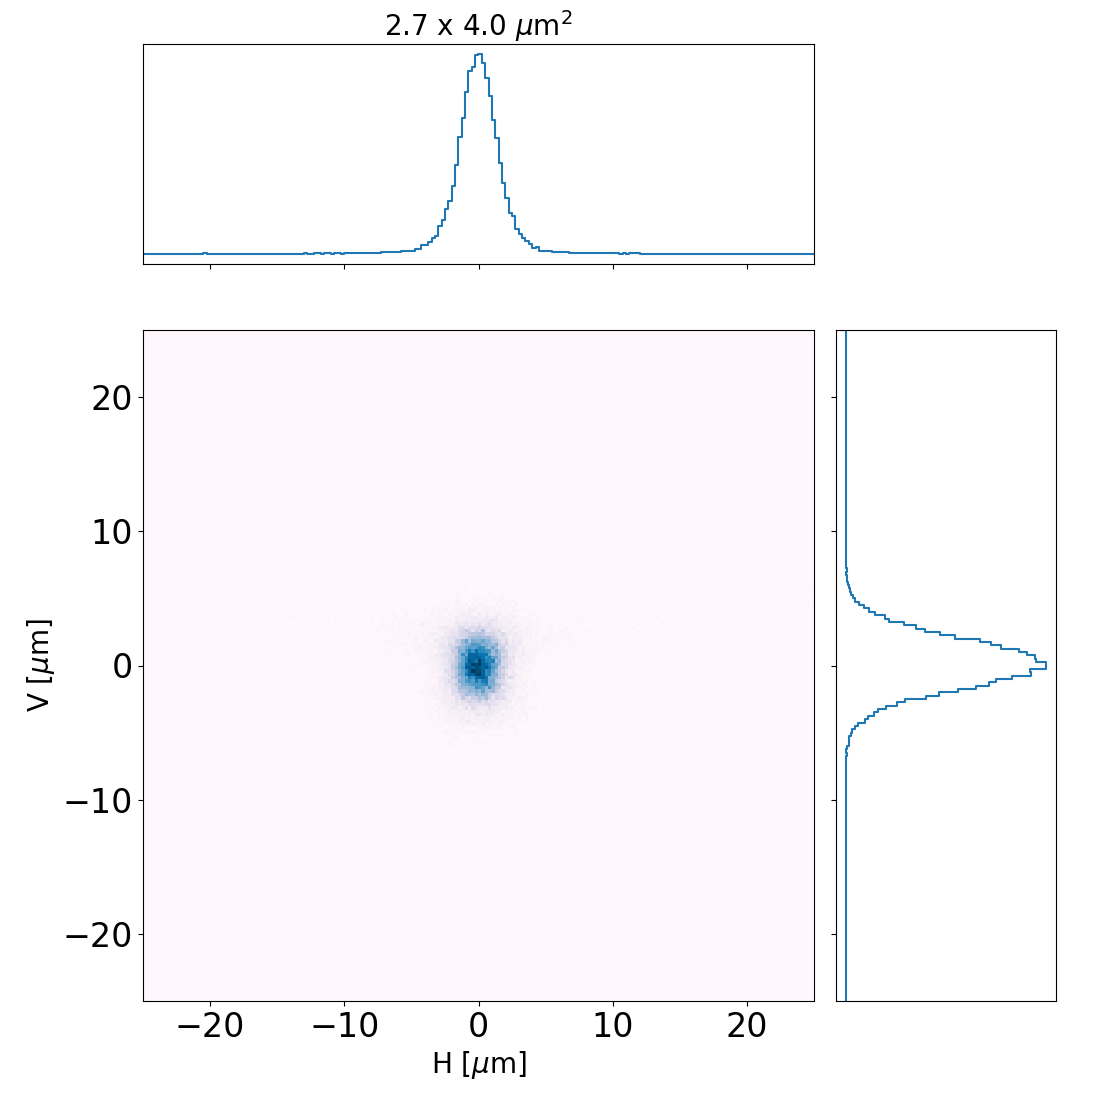
\includegraphics[width=0.32\textwidth]{figures/M0p1_diaboloid.png}
\caption{\label{fig:demagnification}
Image produced by the beamline for two high demagnification values: 1:5 (top) and 1:10 (bottom) using different M2 shapes: a) Toroid, b) Parabolic-cone) and c) Diaboloid.}
\end{figure}


To study in more detail the aberrations, ray-tracing calculations are performed scanning the magnification factor and extracting the focal dimensions. For each ray-tracing simulation this focal dimension is calculated in two ways: i) the FWHM of the intensity distribution (as discussed previously), and ii) the standard deviation $\sigma$ of the ray coordinates contributing to the focal image. The purpose is to evaluate the aberrations by comparing the FWHM with $\sigma$. If the intensity distribution is Gaussian, we will obtain a $\sigma$ smaller than the FWHM by a factor 2.35. However, when aberrations are present the long tails make that the $\sigma$ increases rapidly becoming even greater than the FWHM value. If this happens it is an indicator of high aberrations.  

\begin{figure}[h]
\flushleft
a)~~~~~~~~~~~~~~~~~~~~~~~~~~~~~~~~~~~~~~~~~~~b)~~~~~~~~~~~~~~~~~~~~~~~~~~~~~~~~~~~~~~~~~~~c)\\
\centering
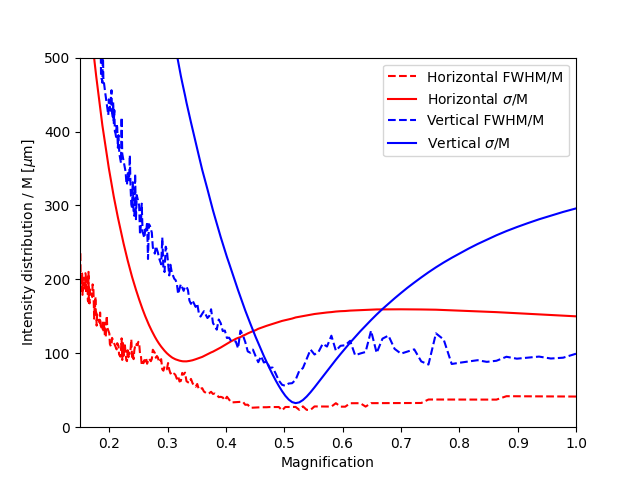
\includegraphics[width=0.32\textwidth]{figures/scan_toroid.png}
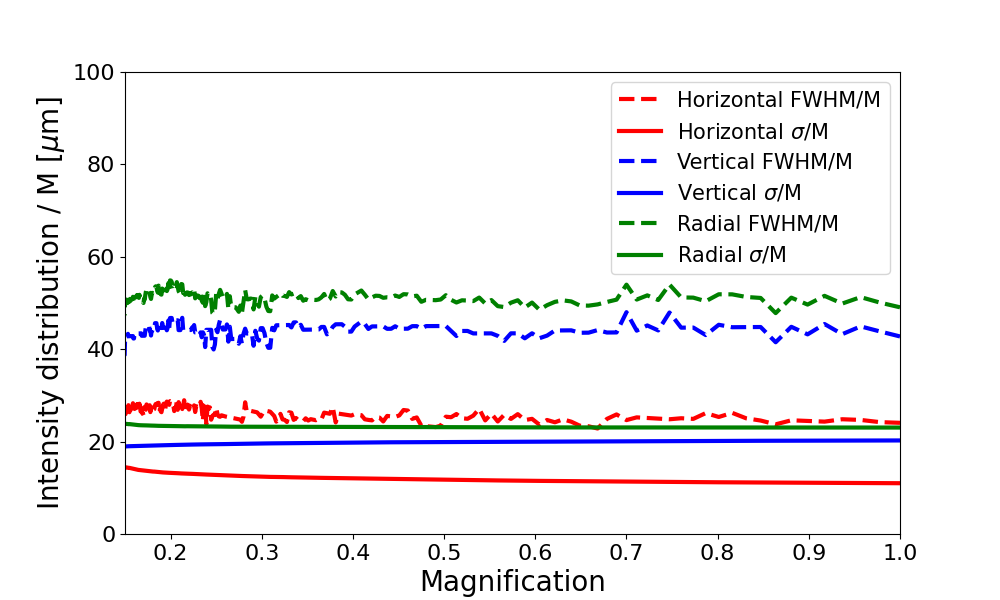
\includegraphics[width=0.32\textwidth]{figures/scan_diaboloid.png}
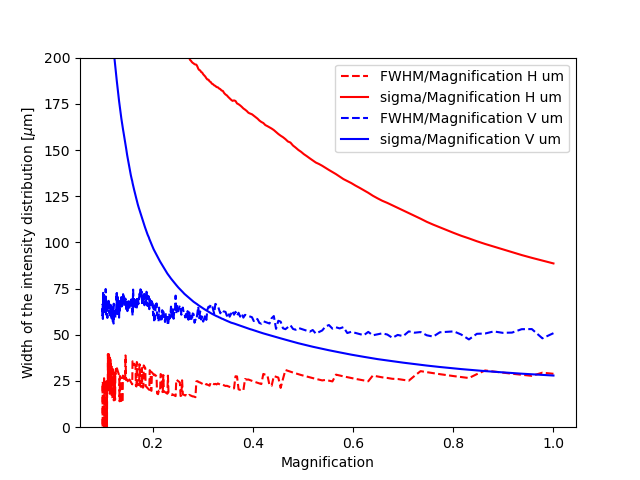
\includegraphics[width=0.32\textwidth]{figures/scan_parabolic-cone.png}

\caption{\label{fig:scan}
Evolution of the (horizontal and vertical) focal size (measured in FWHM and $\sigma$) versus magnification for a beamline with focusing M2 mirror shape: a) toroid, b) Diaboloid and c) Parabolic-cone. 
}
\end{figure}


Fig.~\ref{fig:scan} shows the results of ray-tracing calculations of the focal size versus magnification M. Because the size is proportional to the magnification (in the ideal case of zero aberrations), we have visualized the focal size (in FWHM or $\sigma$ for horizontal and vertical directions) divided by the magnification in order to obtain an constant value in the ideal case of zero aberrations. Looking at the response of the toroidal mirror we can identify large aberrations for most cases (the $\sigma$ values are higher than the FWHM) and there is an optimum value around M=0.5 where the vertical size is minimum. This is the "working condition" of most beamlines using toroids at ALS as the aberrations are minimized \cite{padmore2000,howells2000}. For the Diaboloid (Fig~\ref{fig:scan}b) the situation is completely different. For most of cases (M>0.2) the lines are almost constant and the $\sigma$'s smaller than the FWHM by a value approaching 2.35, indicating that the Diaboloid behaves as a perfect optics. For the parabolic-cone (Fig~\ref{fig:scan}c) the situation is very close to the Diaboloid when looking at the FWHM values down to the minimum M. When the values of $\sigma$ are higher than FWHM there is presence of residual aberrations. This is true for the horizontal focus, an effect already observed in the previous section, and it is less important for the vertical direction: only for M<0.3 the $\sigma$ becomes higher that the FWHM.  



\section{Summary}
\label{sec:summary}

We implemented the Diaboloid equations in Oasys and use them for different simulations. In a Oasys widget the Diaboloid surface is calculated the "basal-plane" approximation, which allows to use simple formulas (Eqs.~\ref{eqn:diaboloidV}, \ref{eqn:diaboloidK}) directly for numerical simulations. We demonstrated its validity for most practical cases where the focal sizes are larger that 1$\mu$m. 
The exact solution \cite{lacey} is very long and can be used in Mathematica to create files that cal also be used in the Oasys environment, and helped also to evaluate the goodness of the approximation. 
The "parabolic-cone" (Eq.~\ref{eqn:parabolicCone}), an  approximation to the Diaboloid, is also implemented. It may play in the future an important role in applying the Diaboloid concept to new beamlines, because it is probably easier to manufacture and polish to enough quality. We studied these mirrors surfaces applied to the ALS beamline 12.2.2 in its present (ALS) and in the Upgraded configuration (ALS-U). It is manifested the possible interest to migrate to Diaboloid or parabolic-cone solutions for the ALS-U, if they can be built. The use of these new solutions may also improve the beamline performances because they can be used with high demagnification. We showed that magnifications of 1:5 and up to 1:10 may be used with parabolic-cone or diaboloid mirrors for this beamline. 

% We have derived an exact solution of the diaboloid mirror in the form
% \begin{equation}
% \label{eqn:summary_form}
% z(x,y) = - \sqrt{A - B y - C \sqrt{x^2 + (y - D)^2}},
% \end{equation}
% in the coordinate system where the source beam is inclined downward at an angle of $2 \theta$, and $x$ and $y$ are rooted at the mirror center. The complete expression for $z(x,y;p,q,\theta)$ is given in Eq. \ref{eqn:7new_z}. It remains to test this exact expression against existing series representations (from McKinney), and through ray-trace beamline modeling.



     %-------------------------------------------------------------------------
     % The back matter of the paper - acknowledgements and references
     %-------------------------------------------------------------------------

     % Acknowledgements come after the appendices



     % References are at the end of the document, between \begin{references}
     % and \end{references} tags. Each reference is in a \reference entry.

% \begin{references}
% \reference{Author, A. \& Author, B. (1984). \emph{Journal} \textbf{Vol}, 
% first page--last page.}
% \end{references}
%\cite{knuth84}

%% Note added by Overleaf: If using bibtex, remove the "references" environment above, and uncomment the following line.
\referencelist{iucr}


%      %-------------------------------------------------------------------------
%      % TABLES AND FIGURES SHOULD BE INSERTED AFTER THE MAIN BODY OF THE TEXT
%      %-------------------------------------------------------------------------
% 
%      % Simple tables should use the tabular environment according to this
%      % model
% 
% \begin{table}
% \caption{Caption to table}
% \begin{tabular}{llcr}      % Alignment for each cell: l=left, c=center, r=right
%  HEADING    & FOR        & EACH       & COLUMN     \\
% \hline
%  entry      & entry      & entry      & entry      \\
%  entry      & entry      & entry      & entry      \\
%  entry      & entry      & entry      & entry      \\
% \end{tabular}
% \end{table}
% 
%      % Postscript figures can be included with multiple figure blocks
% 
% \begin{figure}
% \caption{Caption describing figure.}
% 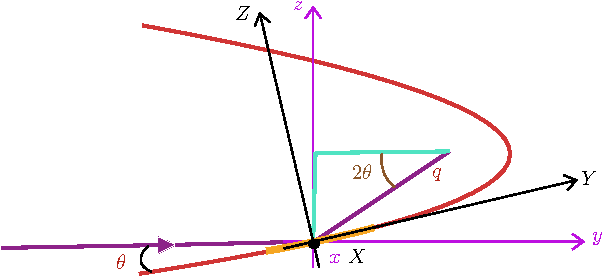
\includegraphics{fig1}
% \end{figure}


\end{document}                    % DO NOT DELETE THIS LINE
%%%%%%%%%%%%%%%%%%%%%%%%%%%%%%%%%%%%%%%%%%%%%%%%%%%%%%%%%%%%%%%%%%%%%%%%%%%%%%


